\documentclass{beamer}

\usepackage[utf8]{inputenc}
\usepackage[french]{babel}
\usepackage{ubuntu}

%% Gestion des figures
\usepackage{graphicx}

\usepackage{caption}
\usepackage{subcaption}
%\setbeamertemplate{caption}[numbered]
\captionsetup{labelformat=simple}
%% Gestion des couleurs
\usepackage{color}

%%%%%%%%%%%%%%%%%%%%%%%%%%%%%%%%%%%%%%%%%%%%%
% Gestion de l'affichage de la presentation %
%%%%%%%%%%%%%%%%%%%%%%%%%%%%%%%%%%%%%%%%%%%%%

%% Theme utilise
\usetheme{warsawpersonalise}%% Une version legerement modiier de warsaw

%% On retire les elements de navigation en bas des frame
\beamertemplatenavigationsymbolsempty

%% Definition des couleurs
	%% Version bleu - marron
\definecolor{haut_fonce}{RGB}{68,116,157}
\definecolor{haut_claire}{RGB}{198,212,225}
\definecolor{bas_fonce}{RGB}{68,116,157}
\definecolor{bas_claire}{RGB}{198,212,225}
\definecolor{block_clair}{RGB}{247,242,242}%{235,231,224}
\definecolor{block_fonce}{RGB}{121,107,96}%{198,212,225}% ou => \definecolor{block_fonce}{RGB}{189,184,173}

	%% Version bleu - marron
% \definecolor{haut_fonce}{RGB}{32,56,120}
% \definecolor{haut_claire}{RGB}{232,216,190}
% \definecolor{bas_fonce}{RGB}{68,116,157}
% \definecolor{bas_claire}{RGB}{198,212,225}
% \definecolor{block_clair}{RGB}{247,242,242}
% \definecolor{block_fonce}{RGB}{157,177,212}% ou => \definecolor{block_fonce}{RGB}{189,184,173}

	%% Version bleu - gris - rouge sang
% \definecolor{haut_fonce}{RGB}{101,114,161}
% \definecolor{haut_claire}{RGB}{162,183,255}
% \definecolor{bas_fonce}{RGB}{133,115,103}
% \definecolor{bas_claire}{RGB}{255,255,255}
% \definecolor{block_clair}{RGB}{202,216,247}
% \definecolor{block_fonce}{RGB}{56,33,18}

\definecolor{fond}{RGB}{255,255,255}

%% Background du canvas
\setbeamercolor{background canvas}{bg=fond}

%% Palette de couleur
% \setbeamercolor{normal text}{fg=haut_fonce}
\setbeamercolor{palette sidebar primary}{use=normal text,fg=normal text.fg}
\setbeamercolor{palette sidebar quaternary}{use=structure,fg=structure.fg}
\setbeamercolor{palette sidebar secondary}{use=structure,fg=structure.fg}
\setbeamercolor{palette sidebar tertiary}{use=normal text,fg=normal text.fg}

\setbeamercolor{structure}{bg=white, fg=block_fonce}

%% Section
\setbeamercolor{section in head/foot}{bg=haut_fonce, fg=white}

%% Sous-section
\setbeamercolor{subsection in head/foot}{bg=haut_claire, fg=white}

%% Footline
\setbeamercolor{footline}{bg=black, fg=black}

%% Block
\setbeamercolor{block title}{bg=block_fonce}
\setbeamercolor{block body}{bg=block_clair}

\setbeamercovered{transparent}
%     abstract
%     abstract title
%     alerted text
%     author
%     author in head/foot
%     author in sidebar
%     background
%     background canvas
%     bibliography entry author
%     bibliography entry location
%     bibliography entry note
%     bibliography entry title
%     bibliography item
%     block body
%     block body alerted
%     block body example
%     block title
%     block title alerted
%     block title example
%     button
%     button border
%     caption
%     caption name
%     date
%     date in head/foot
%     date in sidebar
%     description item
%     enumerate item
%     enumerate subitem
%     enumerate subsubitem
%     example text
%     fine separation line
%     footline
%     framesubtitle
%     frametitle
%     frametitle right
%     headline
%     institute
%     institute in head/foot
%     institute in sidebar
%     item
%     item projected
%     itemize item
%     itemize subitem
%     itemize subsubitem
%     itemize/enumerate body
%     itemize/enumerate subbody
%     itemize/enumerate subsubbody
%     local structure
%     logo
%     lower separation line foot
%     lower separation line head
%     math text
%     math text displayed
%     math text inlined
%     middle separation line foot
%     middle separation line head
%     mini frame
%     navigation symbols
%     navigation symbols dimmed
%     normal text
%     normal text in math text
%     normal text in math text
%     page number in head/foot
%     palette primary
%     palette quaternary
%     palette secondary
%     palette sidebar primary
%     palette sidebar quaternary
%     palette sidebar secondary
%     palette sidebar tertiary
%     palette tertiary
%     part name
%     part title
%     qed symbol
%     quotation
%     quote
%     section in head/foot
%     section in sidebar
%     section in sidebar shaded
%     section in toc
%     section in toc shaded
%     section name
%     section number projected
%     section title
%     separation line
%     sidebar
%     sidebar left
%     sidebar right
%     structure
%     subitem
%     subitem projected
%     subsection in head/foot
%     subsection in sidebar
%     subsection in sidebar shaded
%     subsection in toc
%     subsection in toc shaded
%     subsection name
%     subsection number projected
%     subsection title
%     subsubitem
%     subsubitem projected
%     subsubsection in head/foot
%     subsubsection in sidebar
%     subsubsection in sidebar shaded
%     subsubsection in toc
%     subsubsection in toc shaded
%     subsubsection number projected
%     subtitle
%     title
%     title in head/foot
%     title in sidebar
%     titlegraphic
%     titlelike
%     upper separation line foot
%     upper separation line head
%     verse

%%%%%%%%%%%%%%%%%%%%%%%%%%%%%
% Gestion des codes sources %
%%%%%%%%%%%%%%%%%%%%%%%%%%%%%
\usepackage{listings}

%Version en noir et blanc
\definecolor{colKeys}{rgb}{0,0,0}%{0,0,1}
\definecolor{colIdentifier}{rgb}{0,0,0}
\definecolor{colString}{rgb}{0.6,0.6,0.6}
\definecolor{colComments}{RGB}{68,116,157}%\definecolor{colComments}{rgb}{0.4,0.4,0.4}

%Version couleur :
% \definecolor{colKeys}{RGB}{0,0,0}
% \definecolor{colIdentifier}{RGB}{50,50,50}
% \definecolor{colString}{RGB}{0,53,155}%{RGB}{59,0,159}
% \definecolor{colComments}{RGB}{23,207,236}

\lstset{%configuration de listings
%Style generale de l'affichage
     float=hbp,%
     basicstyle=\ttfamily\normalsize, %
     identifierstyle=\color{colIdentifier}, %
     keywordstyle=\color{colKeys}\bf\normalsize, %
     stringstyle=\color{colString}, %
     commentstyle=\color{colComments}\normalsize\it, %
     columns=flexible, %
     tabsize=2, %
     frame=single, %
     extendedchars=true, %
     showspaces=false, %
     showstringspaces=true, %
     numbers=left, %
     numberstyle=\tiny, %
     breaklines=true, %
     breakautoindent=true, %
     captionpos=b,%
     xrightmargin=0cm, %
     xleftmargin=0cm,
% Permet l'utilisation de balise latex, dont le mode math
     texcl,
% Permet l'affichage d'accent dans le code source
     literate =
%   * Lettres a et A
      {à}{{\`a}}1 {â}{{\^a}}1
      {À}{{\`A}}1 {Â}{{\^A}}1
%   * Lettres c et C
      {ç}{{\c{c}}}1
      {Ç}{{\c{C}}}1
%   * Lettres e et E
      {é}{{\'e}}1 {è}{{\`e}}1 {ê}{{\^e}}1 {ë}{{\"e}}1
      {É}{{\'E}}1 {È}{{\`E}}1 {Ê}{{\^E}}1 {Ë}{{\"E}}1
%   * Lettres i et I
      {î}{{\^i}}1 {ï}{{\"i}}1
      {Î}{{\^I}}1 {Ï}{{\"I}}1
%   * Lettres o et O
      {ô}{{\^o}}1
      {Ô}{{\^O}}1
%   * Lettres u et U
      {ù}{{\`u}}1 {û}{{\^u}}1 {ü}{{\"u}}1
      {Ù}{{\`U}}1 {Û}{{\^U}}1 {Ü}{{\"U}}1
}
%environnement pour langage oriente objet
\lstnewenvironment{C++}{%
            \lstset{language=C++
               %permet de modifier l'affichage du code source selon le langage
               %,identifierstyle=\color{blue},keywordstyle=\color{Ckeywords},backgroundcolor=\color{Cbckgd}
                    }}{}
\lstnewenvironment{java}{%
            \lstset{language=Java}
                        }{}
%environnement pour langage web
\lstnewenvironment{php}{%
            \lstset{language=PHP}
                       }{}
\lstnewenvironment{html}{%
            \lstset{language=HTML}
                        }{}
%environnement pour langage SQL
\lstnewenvironment{sql}{%
            \lstset{language=SQL}
                       }{}
%environnement pour langage fonctionnel
\lstnewenvironment{caml}{%
            \lstset{language=Caml}
                       }{}
\lstnewenvironment{lisp}{%
            \lstset{language=Lisp}
                       }{}
\lstnewenvironment{lisp-term}{%
            \lstset{language=Lisp, backgroundcolor=\color{black}, basicstyle=\ttfamily\small\color{white}}
                       }{}
%autre langage
\lstnewenvironment{make}{%
            \lstset{language=make}
                       }{}
\lstdefinelanguage{algo}{
    keywords={plap, tant, que, fin, faire, si, alors, allant, fonction, fonctions, disponibles, sinon, afficher, pour, chaque, sortie, plop},
    comment=[l]//,
    morecomment=[l]//,
    morecomment=[s]{/*}{*/},
    morestring=[b]",
    mathescape= true,
    sensitive=false,
    literate=
%   * Definition des operateurs avec un style mathematique
      {=}{{$\gets$}}1 {==}{{=}}1 {!=}{{$\neq$}}1
      {<=}{{$\leq$}}1 {>=}{{$\geq$}}1
%   * Definition du mot cle debut avec un accent. Il ne peut etre defini avec keywords car l'accent pose probleme 
      {début}{{\color{colKeys}\bf\normalsize d\'ebut}}1
      {Début}{{\color{colKeys}\bf\normalsize D\'ebut}}1
      {DÉBUT}{{\color{colKeys}\bf\normalsize D\'EBUT}}1      
%   * Definition du mot cle entree avec un accent. Il ne peut etre defini avec keywords car l'accent pose probleme 
      {entrée}{{\color{colKeys}\bf\normalsize entr\'ee}}1
      {Entrée}{{\color{colKeys}\bf\normalsize Entr\'ee}}1
      {ENTRÉE}{{\color{colKeys}\bf\normalsize ENTR\'EE}}1  
%   * Definition du mot cle donnees avec un accent. Il ne peut etre defini avec keywords car l'accent pose probleme 
      {données}{{\color{colKeys}\bf\normalsize donn\'ees}}1
      {Données}{{\color{colKeys}\bf\normalsize Donn\'ees}}1
      {DONNÉES}{{\color{colKeys}\bf\normalsize DONN\'EES}}1
%   * Redefinition des lettres accentuees car la definition precedente aura ecrase ces valeurs
%   * Lettres a et A
      {à}{{\`a }}1 {â}{{\^a}}1
      {À}{{\`A }}1 {Â}{{\^A}}1
%   * Lettres c et C
      {ç}{{\c{c}}}1
      {Ç}{{\c{C}}}1
%   * Lettres e et E
      {é}{{\'e}}1 {è}{{\`e}}1 {ê}{{\^e}}1 {ë}{{\"e}}1
      {É}{{\'E}}1 {È}{{\`E}}1 {Ê}{{\^E}}1 {Ë}{{\"E}}1
      {œ}{{\oe}}1 {Œ}{{\OE}}1
%   * Lettres i et I
      {î}{{\^i}}1 {ï}{{\"i}}1
      {Î}{{\^I}}1 {Ï}{{\"I}}1
%   * Lettres o et O
      {ô}{{\^o}}1
      {Ô}{{\^O}}1
%   * Lettres u et U
      {ù}{{\`u}}1 {û}{{\^u}}1 {ü}{{\"u}}1
      {Ù}{{\`U}}1 {Û}{{\^U}}1 {Ü}{{\"U}}1
}
\lstnewenvironment{algo}{%
            \lstset{language=algo}
                       }{}
%pour le langage des machines a registre
\lstdefinelanguage{RAM}{%
    morekeywords={plop, read, write, load, store, jz, decr, incr, jump, stop, plop}
    comment=[l]//,
    morecomment=[l]//,
    morecomment=[s]{/*}{*/},
    mathescape= true,
    sensitive=false
}
\lstnewenvironment{RAM}{%
            \lstset{language=RAM, firstnumber=0}
                       }{}

\title{Réseaux viaires et évacuation}
\author{Thibaut Démare}
\institute{Stage de recherche\\Université du Havre}
\date{\today}

%%%%%%%%%%%%%%%%%%%%%%%%%%%%%% Fin du préambule  %%%%%%%%%%%%%%%%%%%%%%%%%%%%%%%%%%%%%%%%%%%%%%%%%%%%%%%%%%%%%%

%%%%%%%%%%%%%%%%%%%%%%%%%%%%%% Debut du document %%%%%%%%%%%%%%%%%%%%%%%%%%%%%%%%%%%%%%%%%%%%%%%%%%%%%%%%%%%%%%
\begin{document}

\begin{frame} 
\titlepage
\end{frame}

\section{A context of evacuation}

	\subsection{A complex system}
	
\begin{frame}{Le Havre - A complex system}
	\begin{figure}[htbp]
		\centering
		\subcaptionbox{A manifestation of Royal de Luxe.}[0.48\linewidth][c]{
			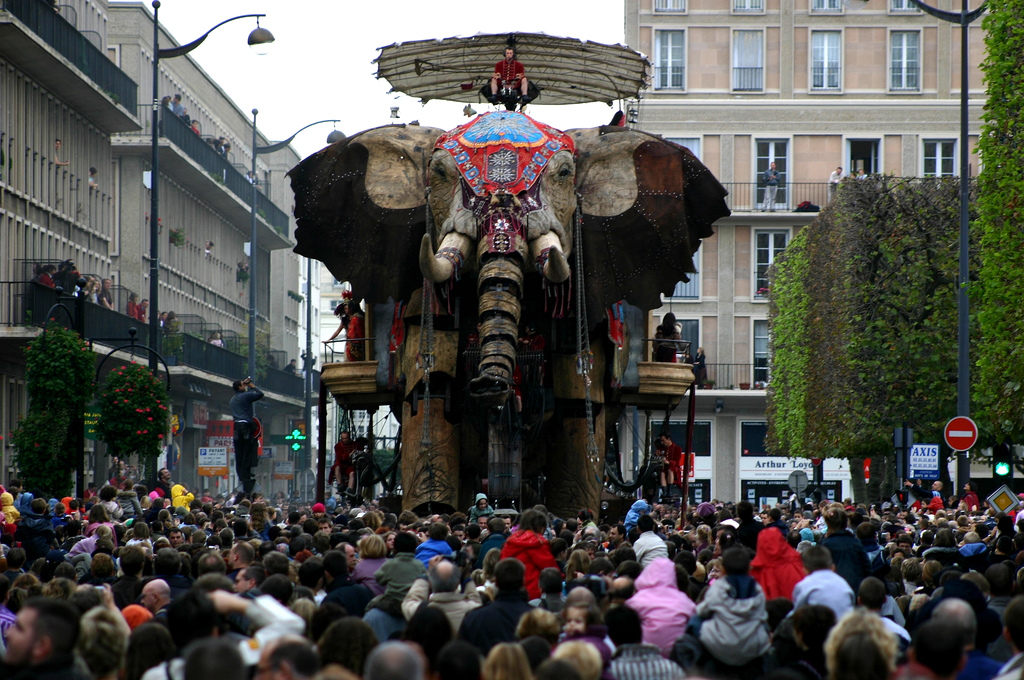
\includegraphics[width=0.48\linewidth]{./img/le_havre_system_complex_human.jpg}
		}
		\subcaptionbox{A herring gull.}[0.48\linewidth][c]{
			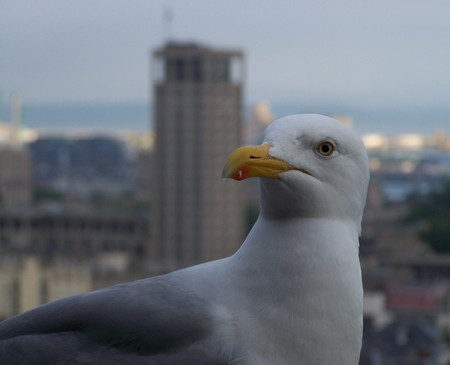
\includegraphics[width=0.48\linewidth]{./img/le_havre_system_complex_animal.jpg}
		}
		\caption{Many interactions in the complex system.}
		\label{fig:complex_systems_1}
	\end{figure}
\end{frame}

\begin{frame}{Le Havre - A complex system}
	\begin{figure}[htbp]
		\centering
		\subcaptionbox{Seine's estuary.}[0.48\linewidth][c]{
			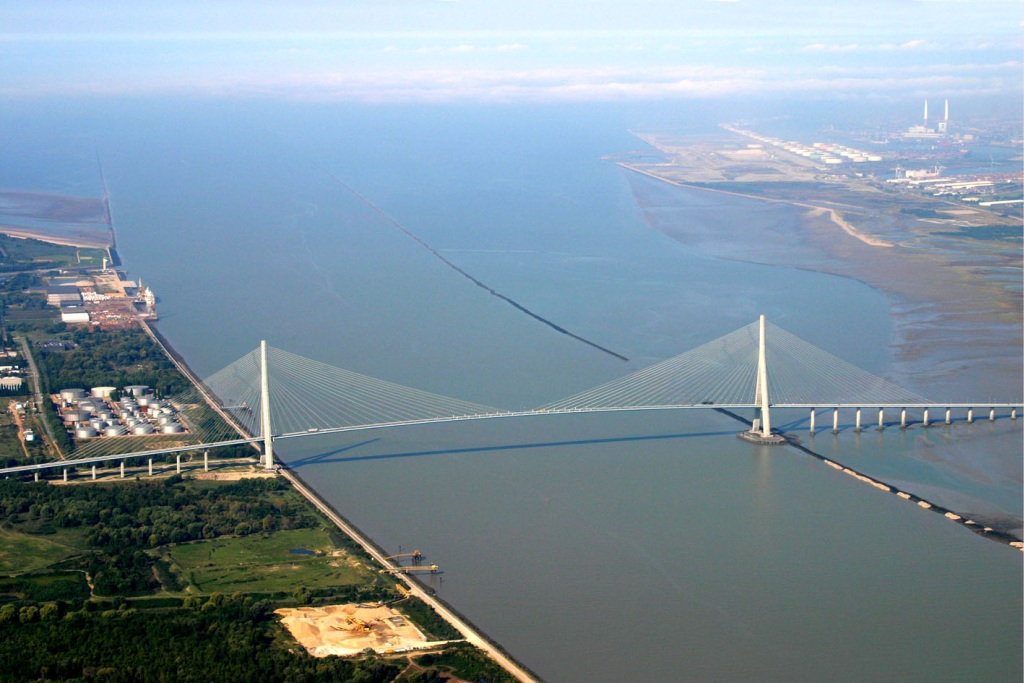
\includegraphics[width=0.48\linewidth]{./img/le_havre_system_complex_environnement.jpg}
		}
		\subcaptionbox{Port of Le Havre.}[0.48\linewidth][c]{
			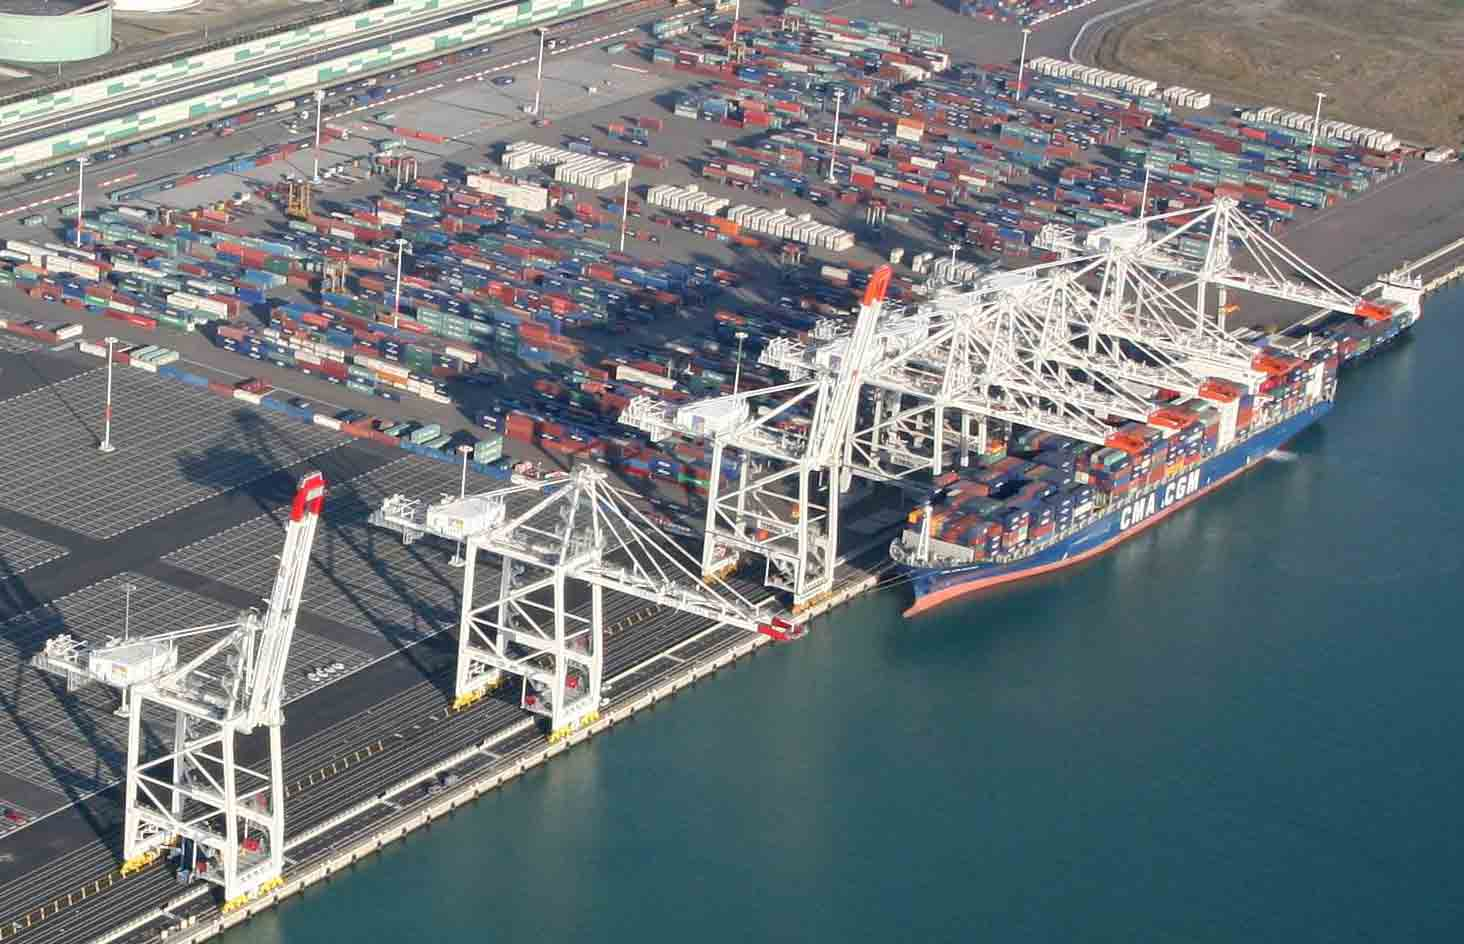
\includegraphics[width=0.48\linewidth]{./img/le_havre_system_complex_port.jpg}
		}
		\caption{Many interactions in the complex system.}
		\label{fig:complex_systems_2}
	\end{figure}
\end{frame}

\begin{frame}{Le Havre - Problems and a difficult management of roads}
	\begin{figure}[htbp]
		\centering
		\subcaptionbox{Bottleneck on Boulevard Winston Churchill.}[0.48\linewidth][c]{
			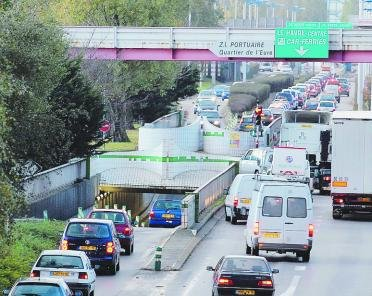
\includegraphics[width=0.48\linewidth]{./img/le_havre_problem_transport.jpg}
		}
		\subcaptionbox{Industries involve major risks.}[0.48\linewidth][c]{
			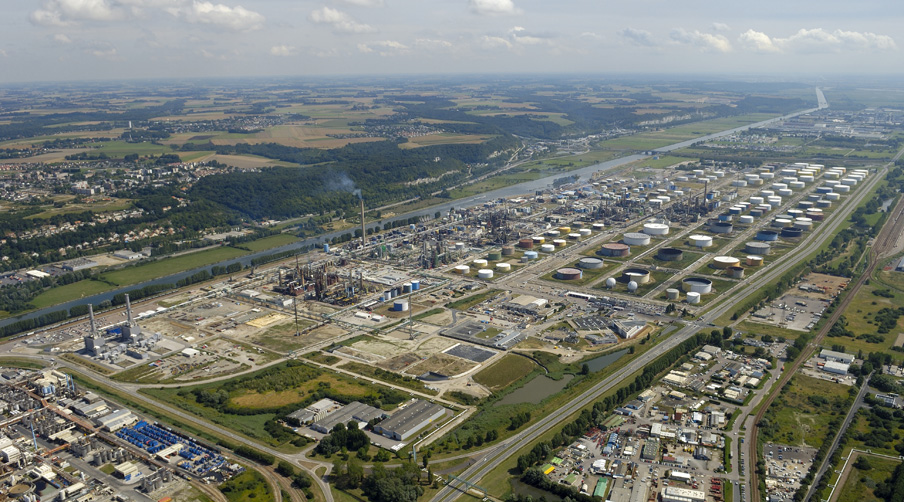
\includegraphics[width=0.48\linewidth]{./img/le_havre_problem_industries.jpg}
		}
		\caption{Needs to define second itineraries.}
		\label{fig:problem_and_difficulties}
	\end{figure}
\end{frame}

	\subsection{Toward the graph theory}
	
\begin{frame}{From a city to a road network}
	\begin{figure}[htbp]
		\centering
		\subcaptionbox{Satellite view of the agglomeration of Le Havre.}[0.47\linewidth][c]{
			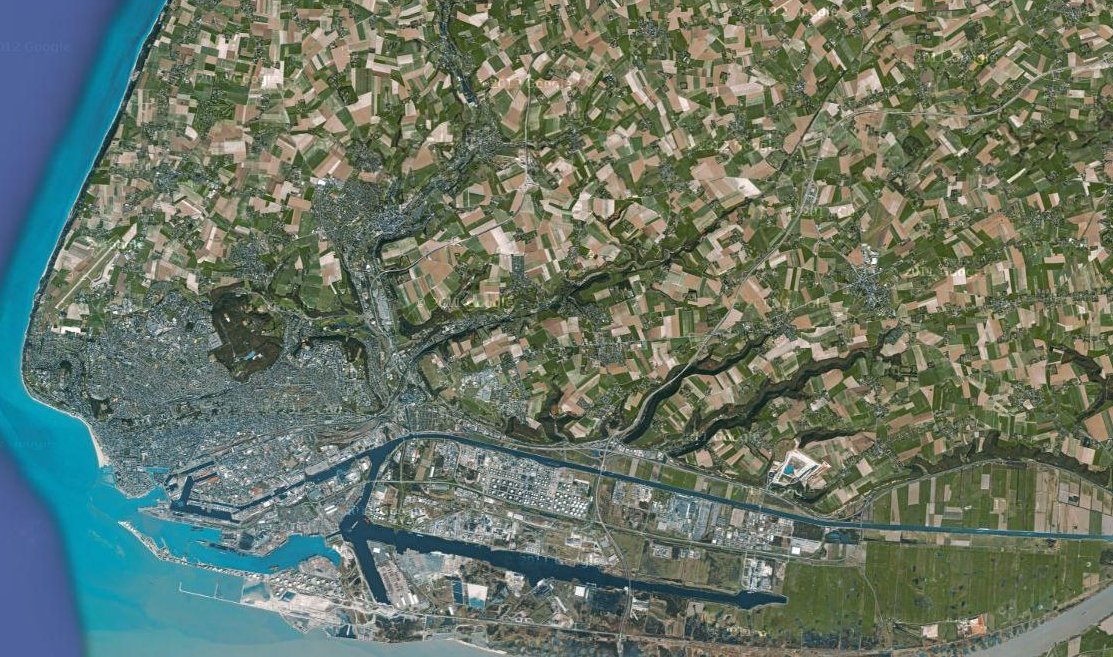
\includegraphics[width=0.47\linewidth]{./img/satellite_view_le_havre.png}
		}
		$\Rightarrow$
		\subcaptionbox{The road network of Le Havre.}[0.47\linewidth][c]{
			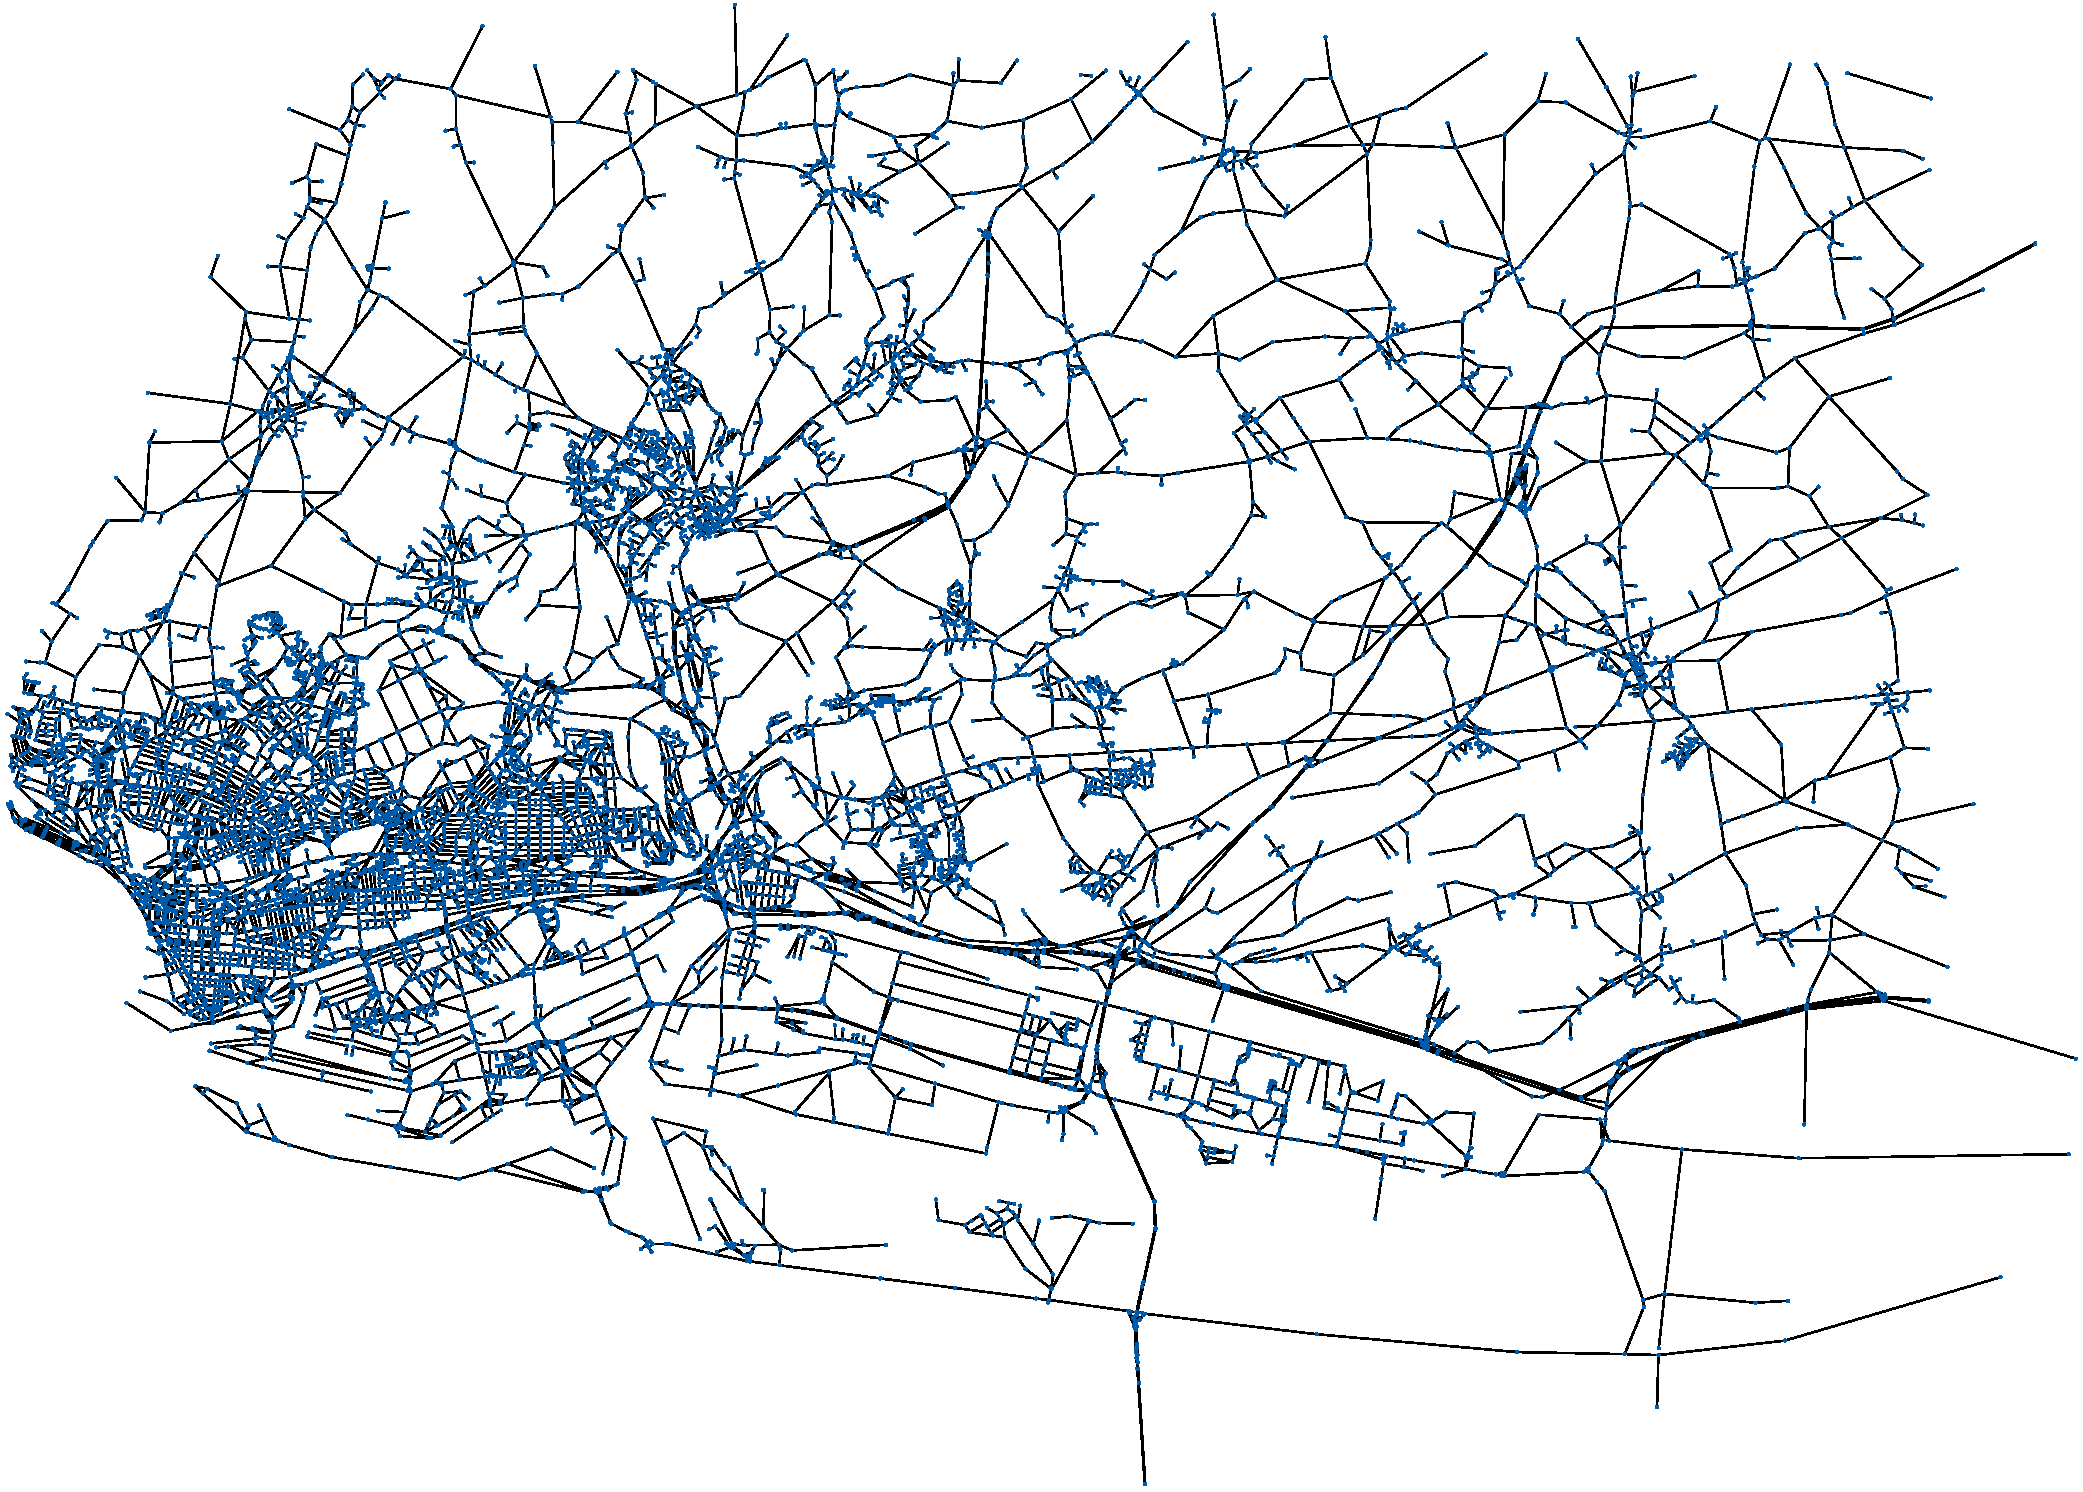
\includegraphics[width=0.47\linewidth]{./img/screenshot_Le_Havre.pdf}
		}
		\caption{Use of the graph theory in order to model the roads of Le Havre and his agglomeration.}
		\label{fig:to_a_network}
	\end{figure}
\end{frame}

\begin{frame}{Measures with the intention of identifying critical areas}
	\begin{figure}[htbp]
		\centering
		\subcaptionbox{Degree centrality.}[0.49\linewidth][c]{
			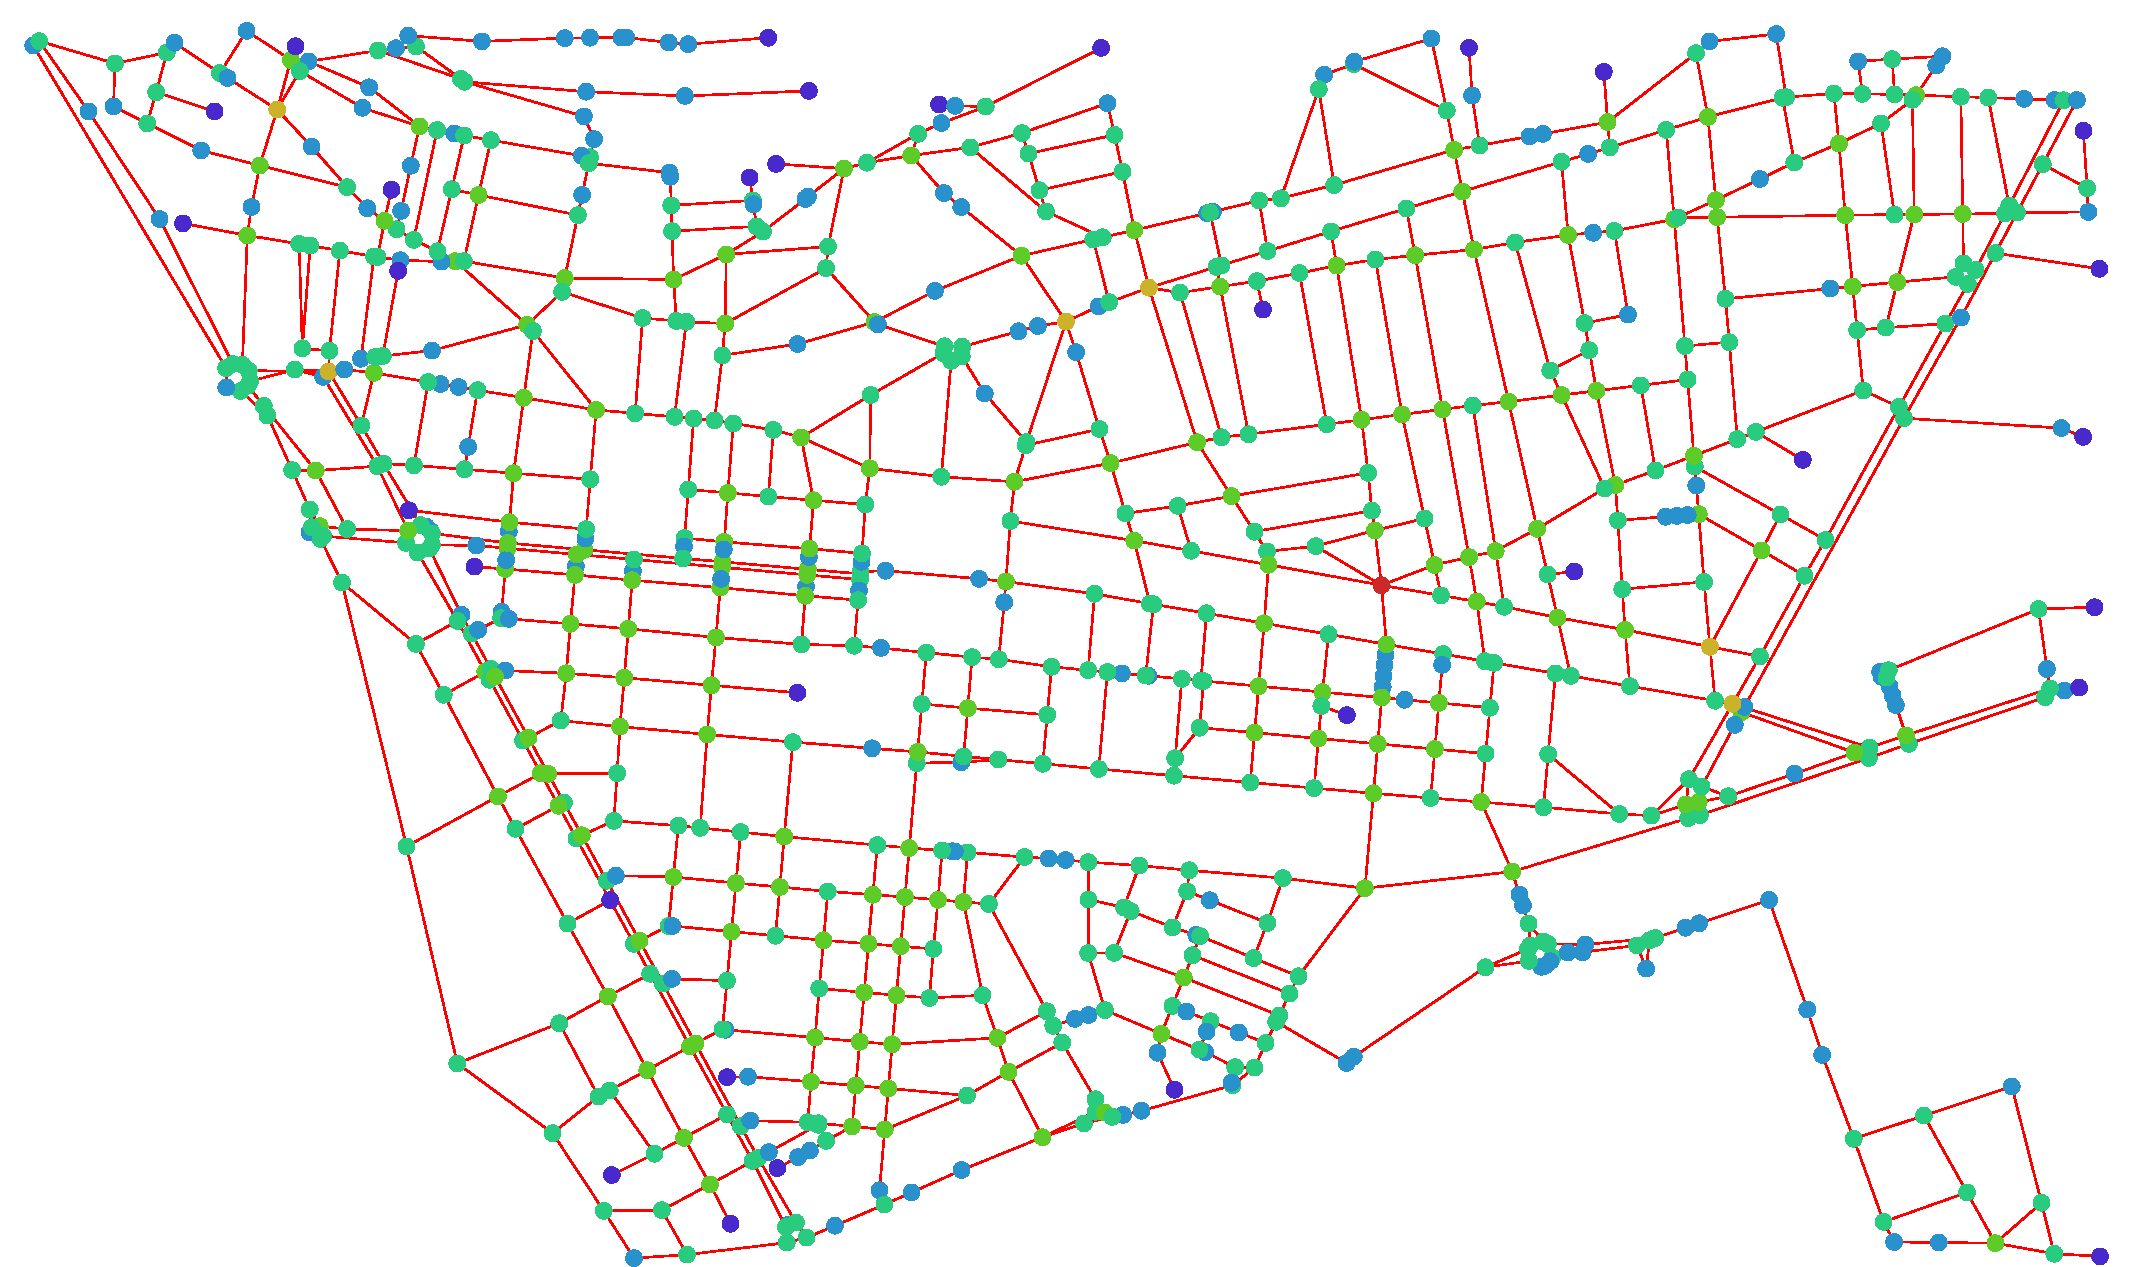
\includegraphics[width=0.49\linewidth]{./img/degree_centrality.pdf}
		}
		\hfill
		\subcaptionbox{Maximum farness centrality.}[0.49\linewidth][c]{
			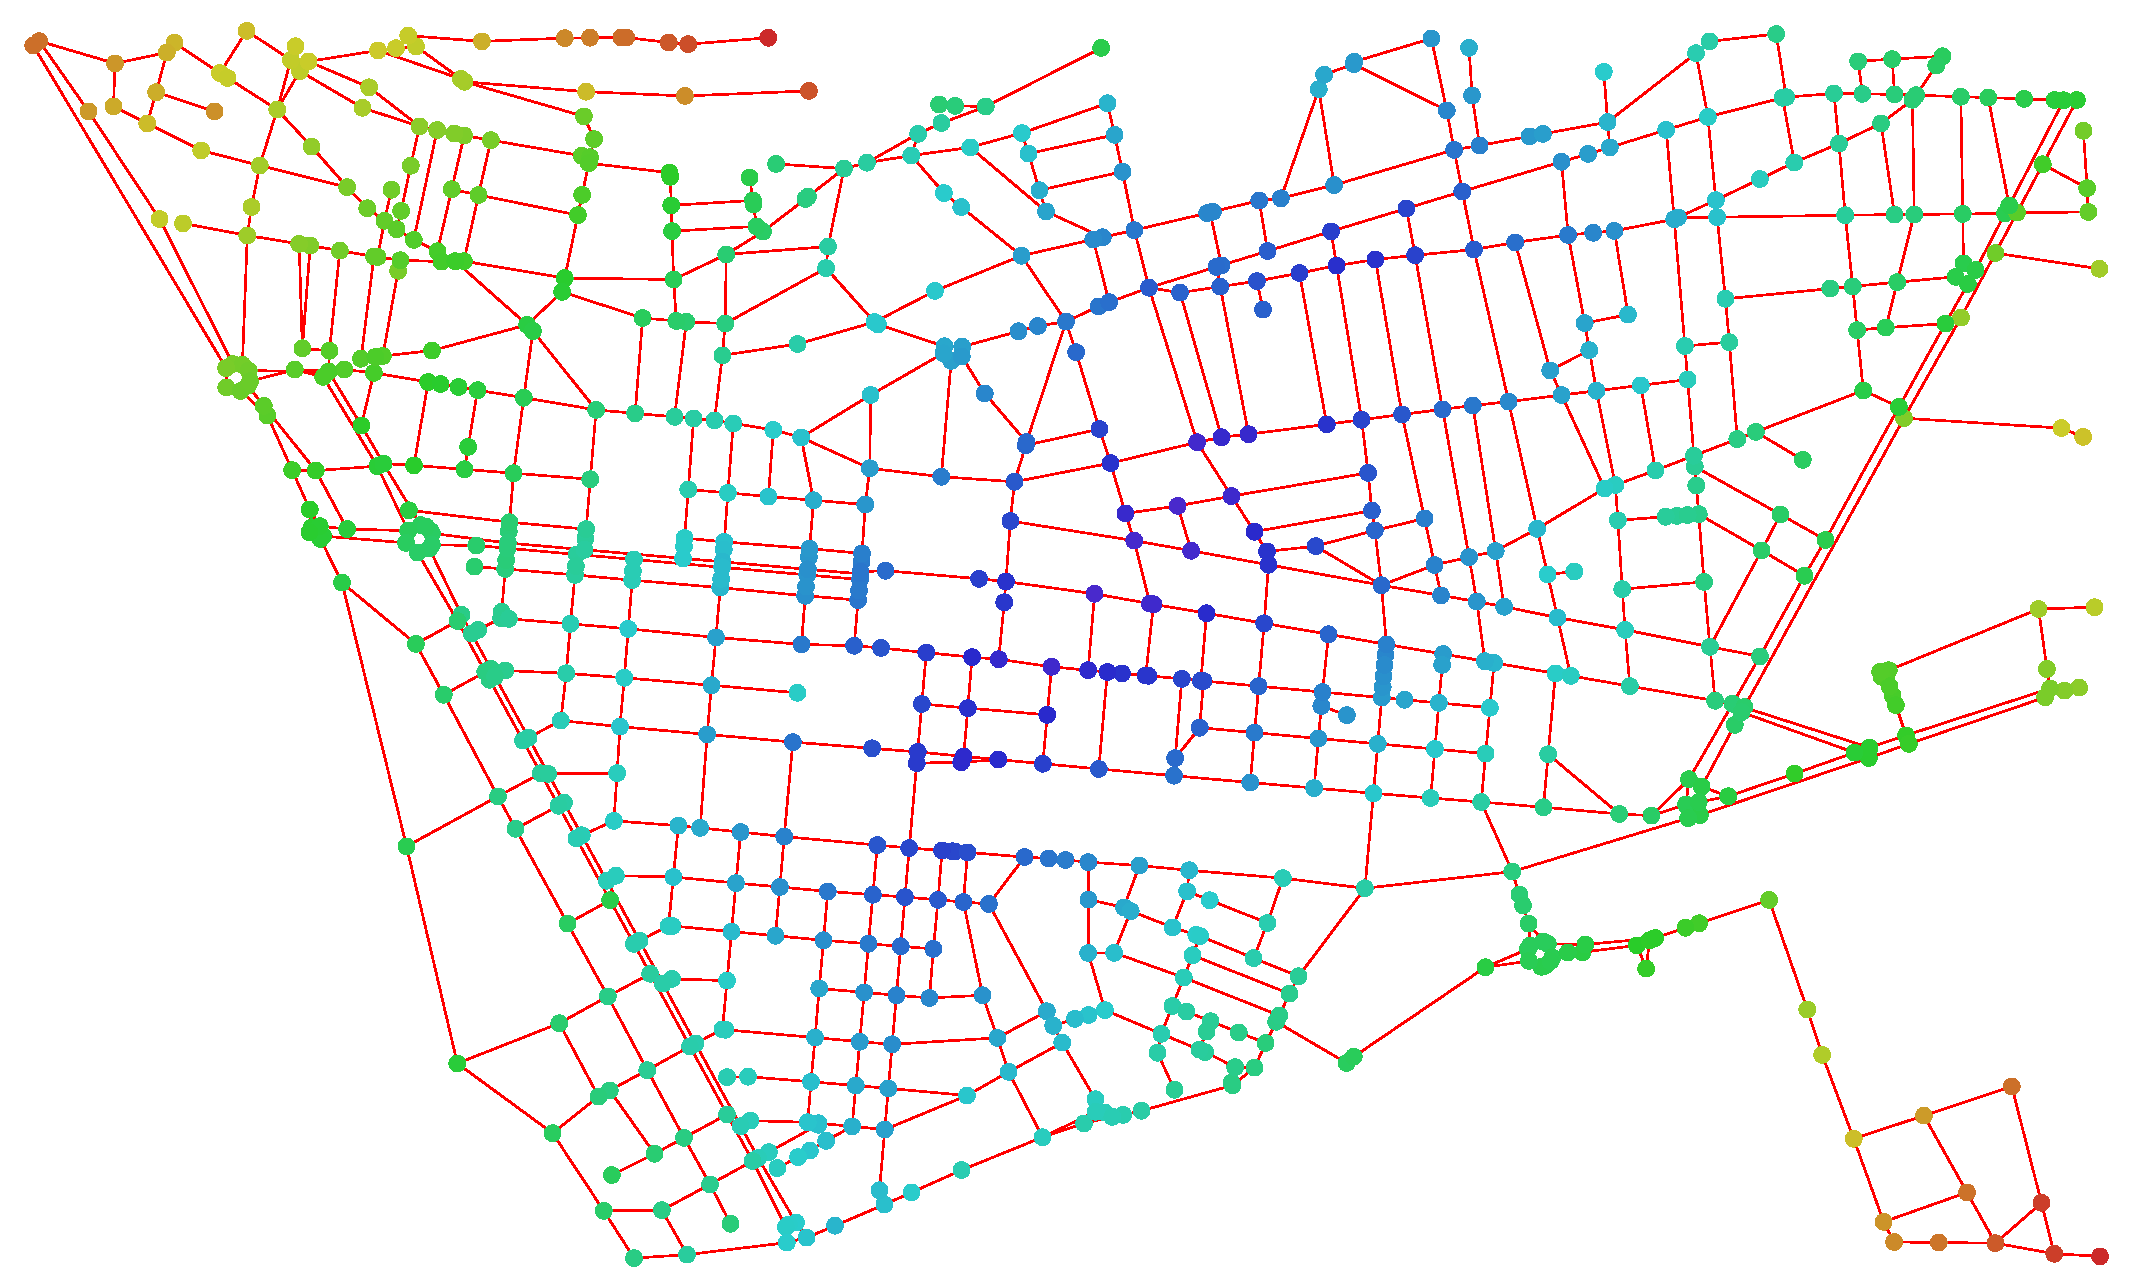
\includegraphics[width=0.49\linewidth]{./img/max_farness_centrality.pdf}
		}
		\caption{Different centralities of the partial and simplified network of Le Havre. From high measures in red to low measures in blue.}
		\label{fig:centralities_1}
	\end{figure}
\end{frame}

\begin{frame}{Measures with the intention of identifying critical areas}
	\begin{figure}[htbp]
		\centering
		\subcaptionbox{Closeness centrality.}[0.49\linewidth][c]{
			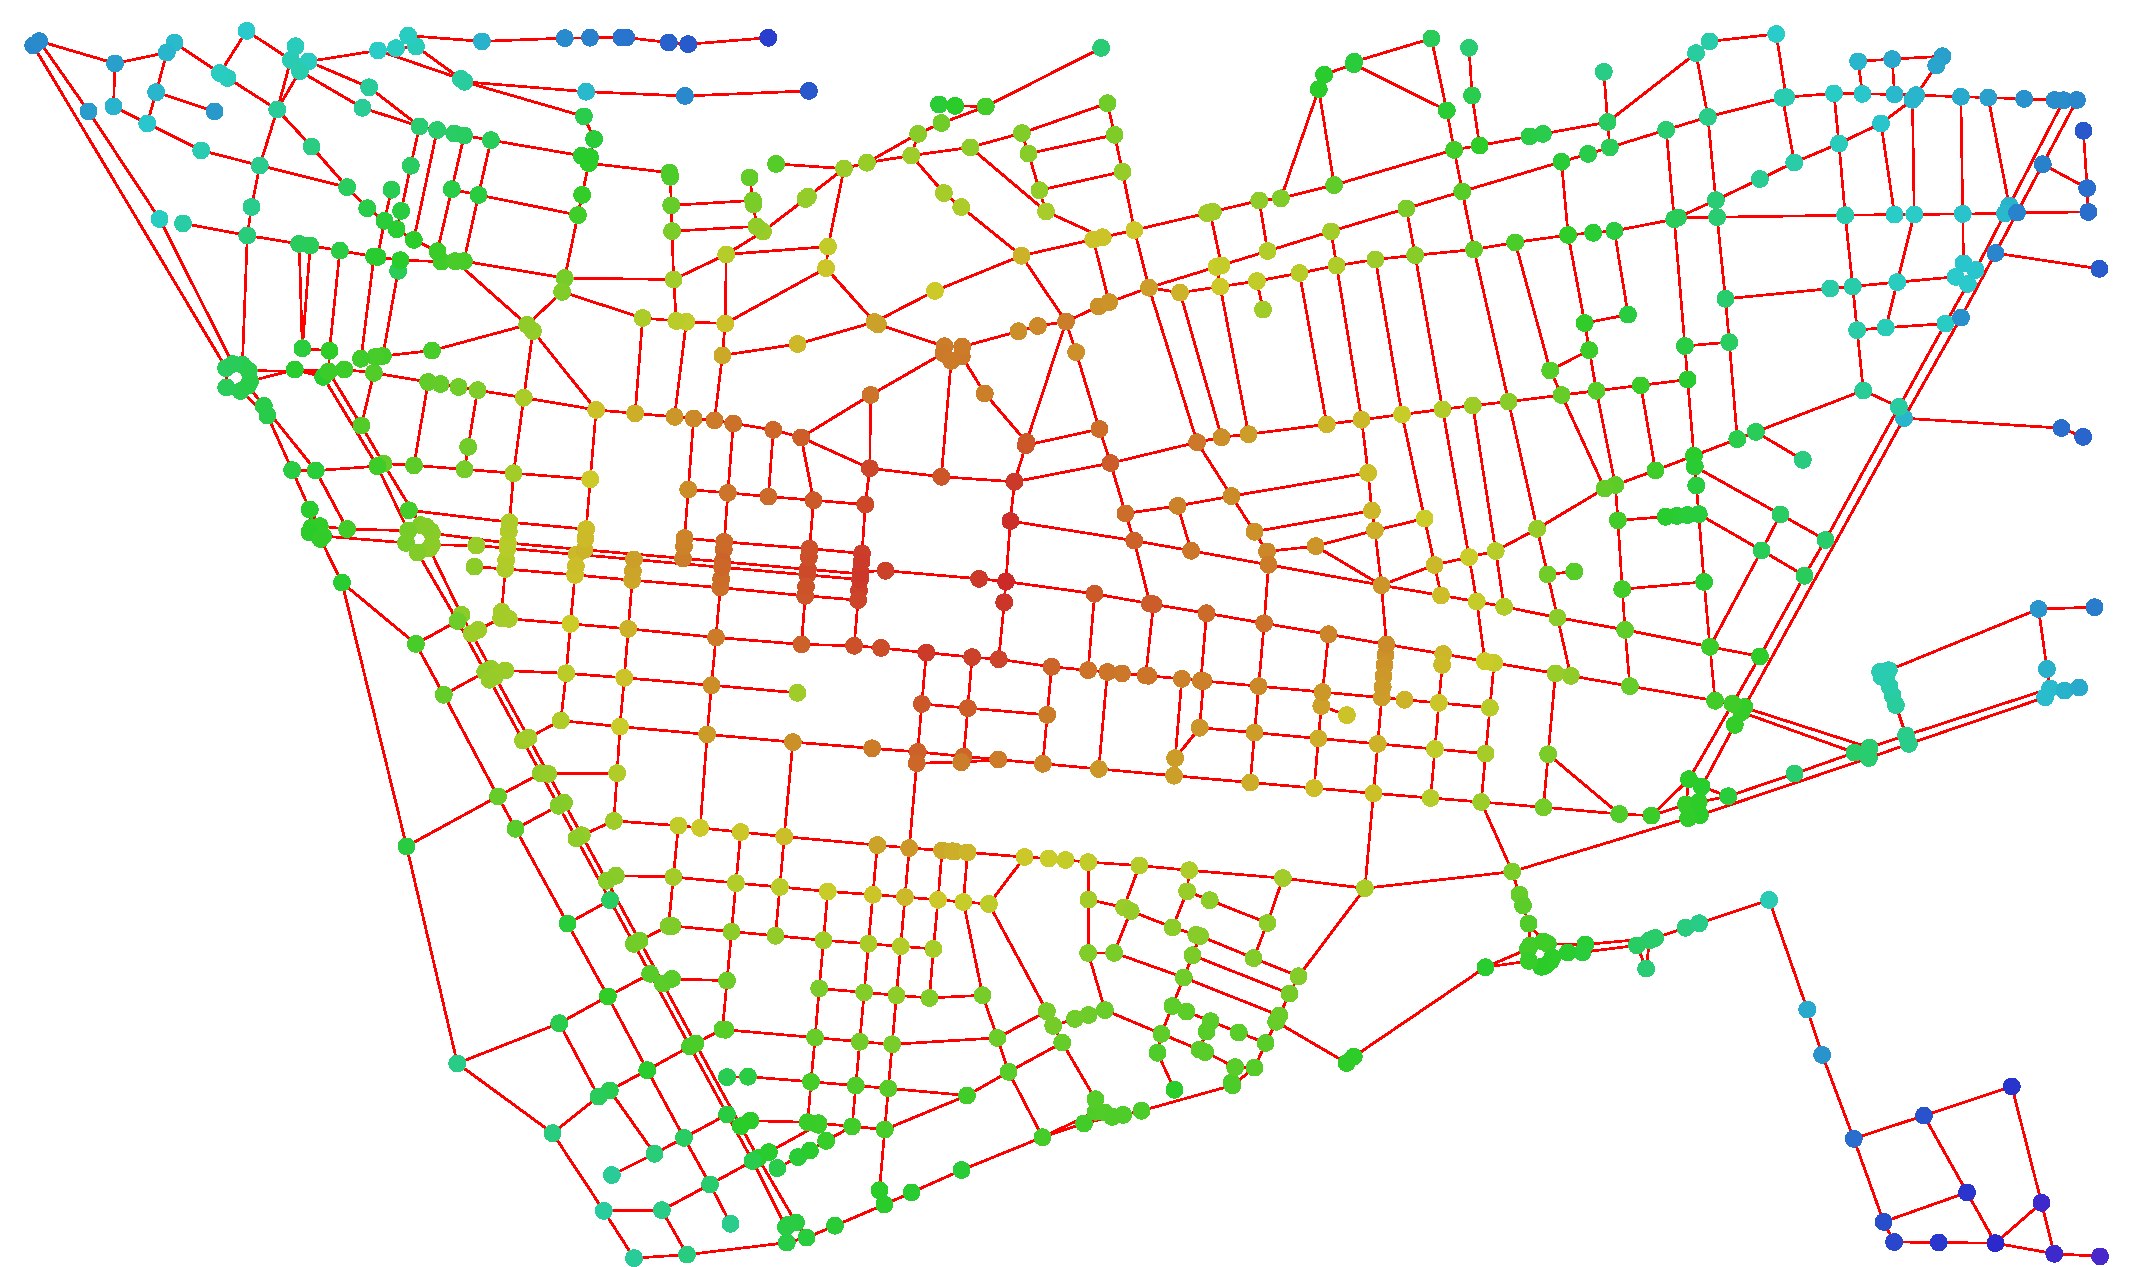
\includegraphics[width=0.49\linewidth]{./img/closeness_centrality.pdf}
		}
		\hfill
		\subcaptionbox{Betweenness centrality.}[0.49\linewidth][c]{
			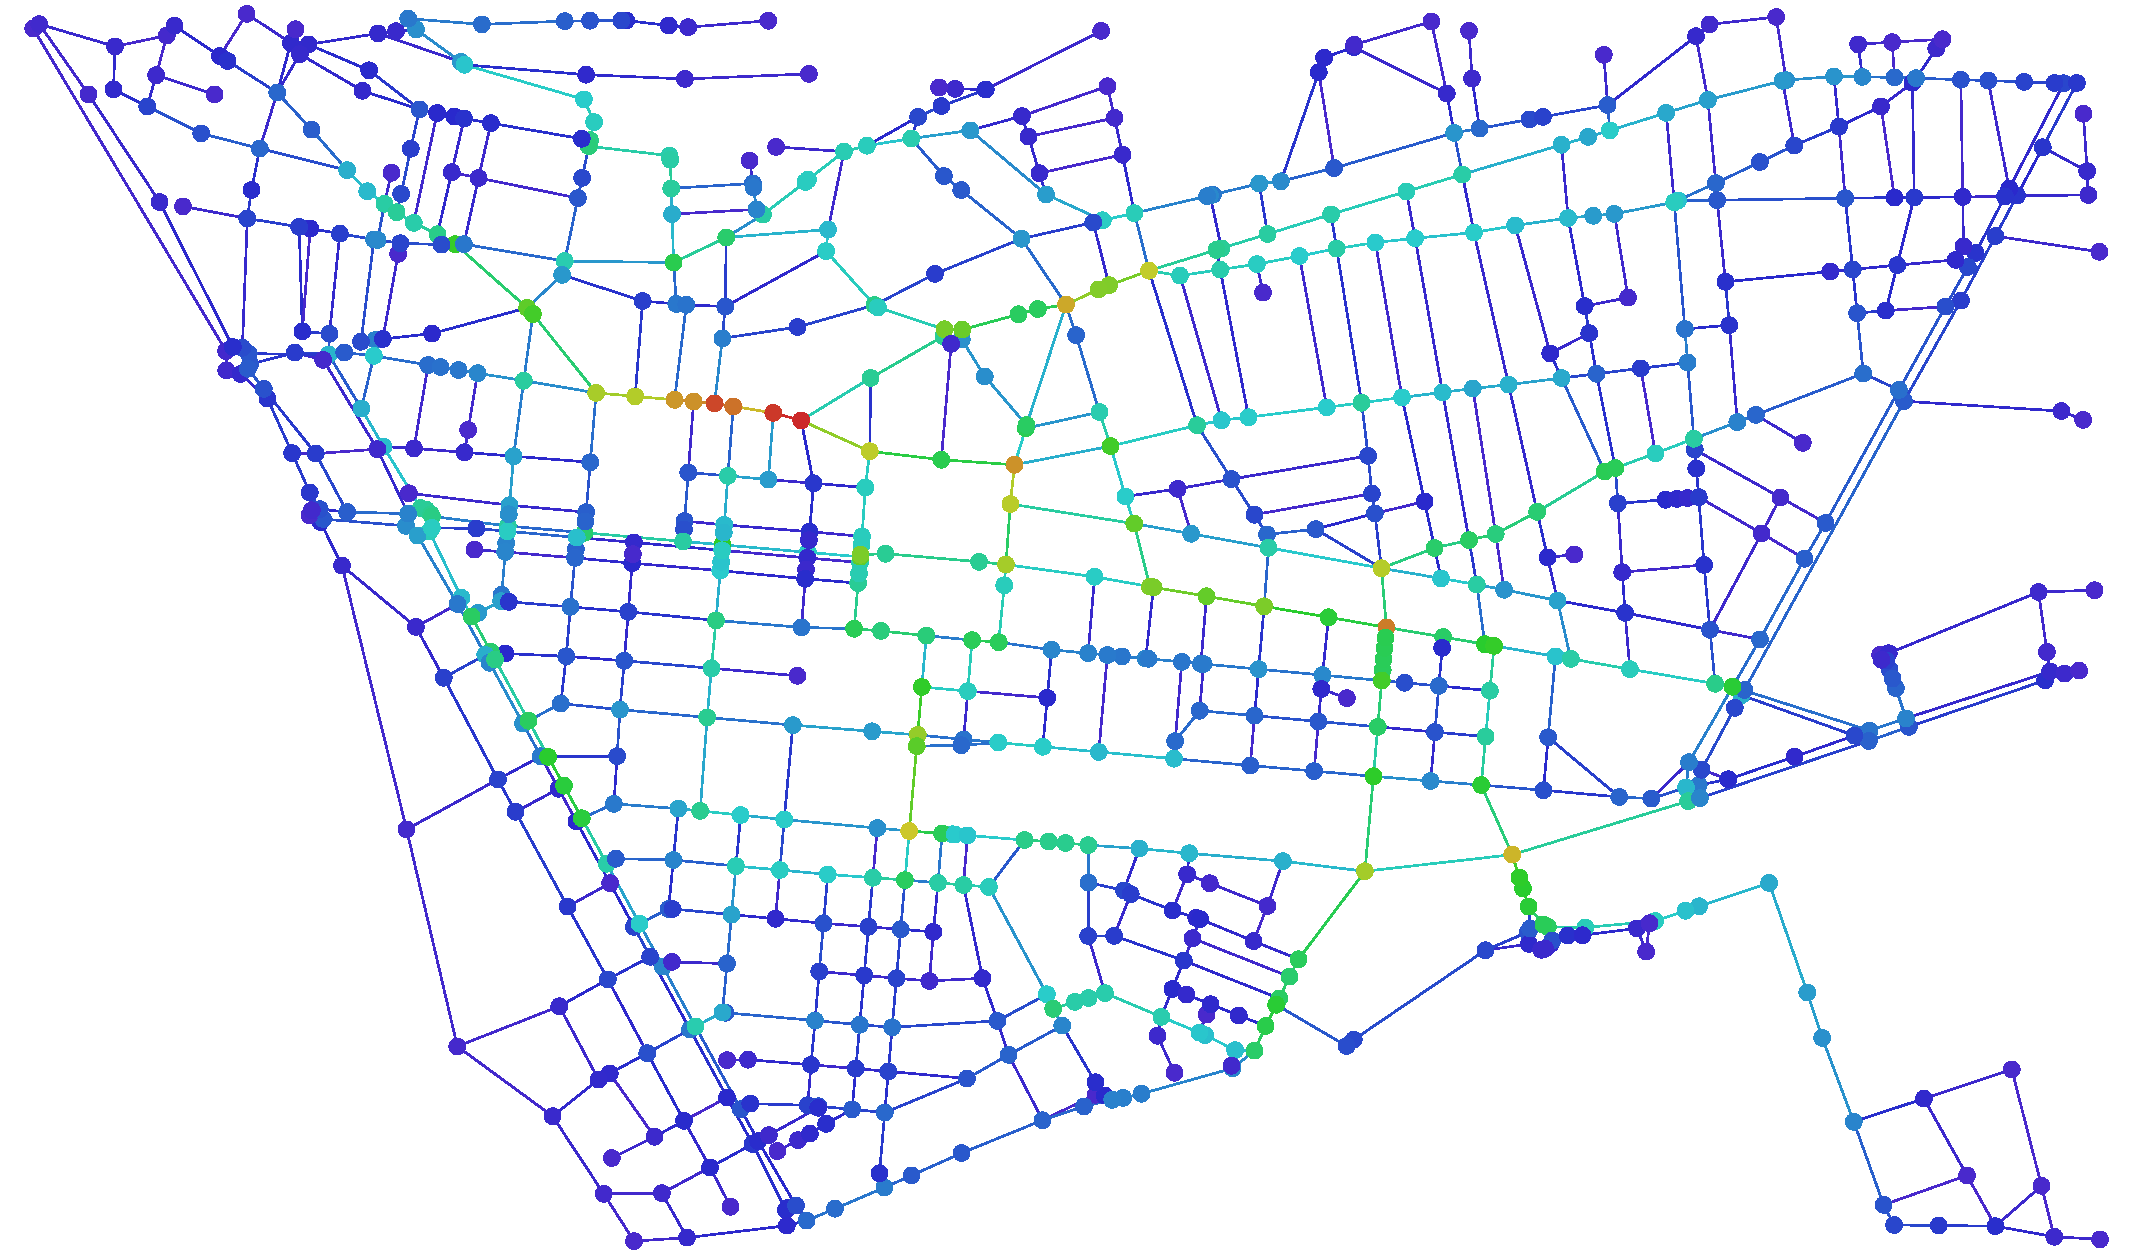
\includegraphics[width=0.49\linewidth]{./img/betwenness_centrality.pdf}
		}
		\caption{Different centralities of the partial and simplified network of Le Havre. From high measures in red to low measures in blue.}
		\label{fig:centralities_2}
	\end{figure}
\end{frame}

	\subsection{A problem of dynamic}
	
\begin{frame}{And in a dynamic system?}
	\begin{block}{where are the dynamics?}
		\begin{itemize}
			\item A road accident which paralyzes the traffic : Wishes to drive around the accident and avoid creating a bottleneck.
			\item An industrial accident which, for example, generates a toxic wind : The areas is to evacuate quickly.
		\end{itemize}
		A part of the network can disappear. A set of nodes and edge can become inaccessible or can be deleted.
	\end{block}
\end{frame}

\begin{frame}{And in a dynamic system?}
	\begin{block}{What are the need and the problem?}
		\begin{itemize}
			\item The need : we want to update the measure in order to have a new idea of the state of the network.
			\item The problem : it is very slow and very expensive to compute.
		\end{itemize}
	\end{block}
\end{frame}

\begin{frame}
	\begin{center}
		We need robust methods for the dynamic !
	\end{center}
\end{frame}

\begin{frame}<beamer>
    \frametitle{Plan}
		%\tableofcontents[currentsection]
		\begin{columns}[t]
			\begin{column}{5cm}
				\tableofcontents[sections={1-2}]
			\end{column}
			\begin{column}{5cm}
				\tableofcontents[sections={3-5}]
			\end{column}
		\end{columns}
\end{frame}


\section{La centralité intermédiaire}

\AtBeginSubsection[] 
{
	\begin{frame}<beamer>
		\addtocounter{framenumber}{-1}
		\frametitle{Plan}
		%\tableofcontents[currentsection]
		\begin{columns}[t]
			\begin{column}{5cm}
				\tableofcontents[sections={1-2},currentsection, currentsubsection, hideothersubsections, subsectionstyle=show/shaded]
			\end{column}
			\begin{column}{5cm}
				\tableofcontents[sections={3-5},currentsection, currentsubsection, hideothersubsections, subsectionstyle=show/shaded]
			\end{column}
		\end{columns}
	\end{frame}
}

	\subsection{Définition et méthode de calcul}
	
\begin{frame}{La centralité intermédiaire (Freeman, 1977)}
	\begin{block}{Définition}
		\begin{itemize}
		    \item<1-> $G=(V, E)$ un graphe, tel que $V$ est l'ensemble de ses sommets avec $n=|V|$, $E$ est l'ensemble de ses arcs avec $m=|E|$. 
			\item<2-> $g_{st}(k)$ est le nombre de plus courts chemins entre $s$ et $t$ passant par $k$.
			\item<3-> $g_{st}$ est le nombre de plus courts chemins entre $s$ et $t$.
			$$
				C_{B}(k)=\underset{s\neq t\neq k}{\sum_s^{n}\sum_t^{n}}\frac{g_{st}(k)}{g_{st}}
			$$
		\end{itemize}
	\end{block}
\end{frame}

\begin{frame}{L'algorithme de calcul (Brandes, 2001)}
	\begin{figure}[htbp]
		\centering
		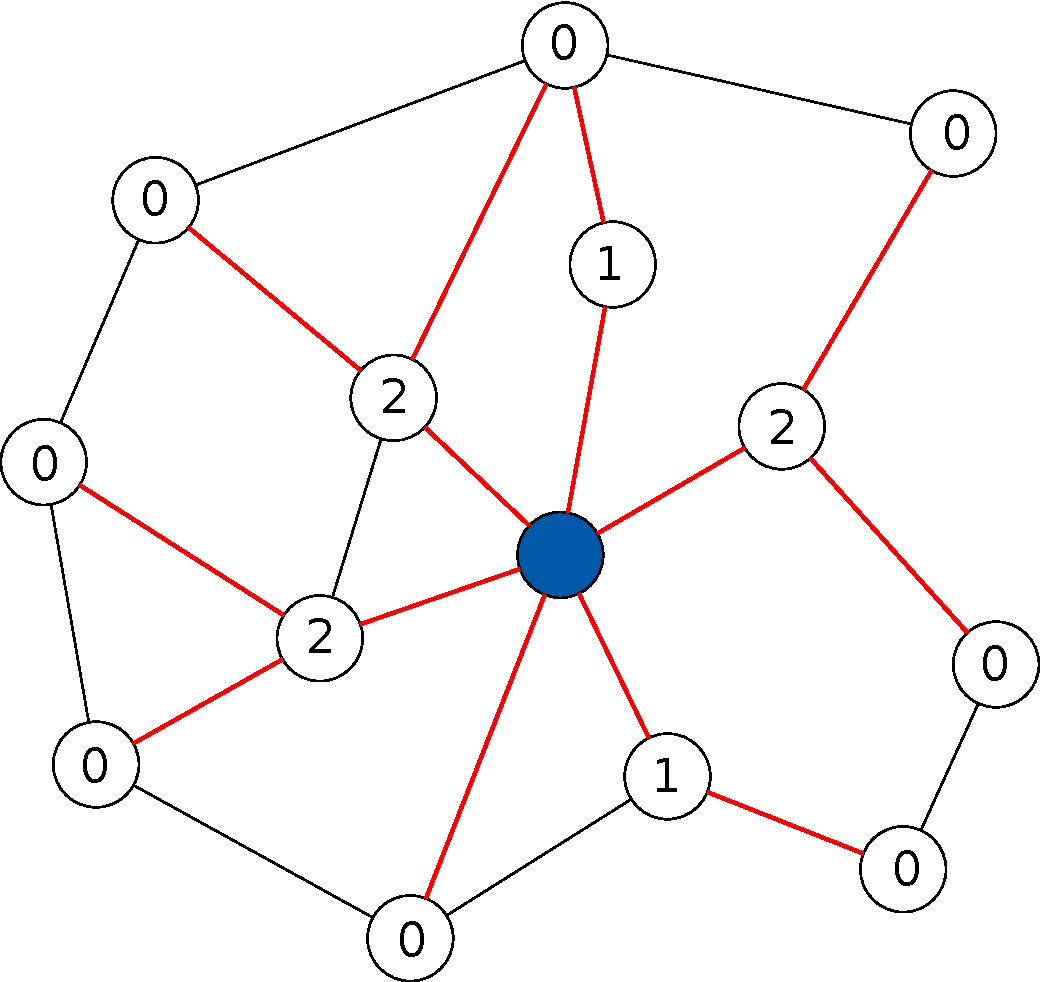
\includegraphics[width=0.49\linewidth]{./img/algo_brandes.pdf}
		\caption{Création des chemins en partances d'un n\oe ud, puis accumulation de la centralité.}
		\label{fig:algo_brandes}
	\end{figure}
\end{frame}

	\subsection{Variantes}

\begin{frame}
	\begin{block}{Quelques variantes}
		\begin{itemize}
		    \item<1-> Utilisation des flots (Freeman \textit{et al.}, 1991) : les chemins font partie d'une solution de flots maximales.
		    \item<2-> K-centralité intermédiaire (Borgatti \textit{et al.}, 2006): recherche des chemins dont la taille est bornée par K.
		    \item<3-> Utilisation de marches aléatoires (Newman, 2005) : les chemins sont déterminés par une marche aléatoire.
		    
		    \begin{figure}[htbp]
				\centering
				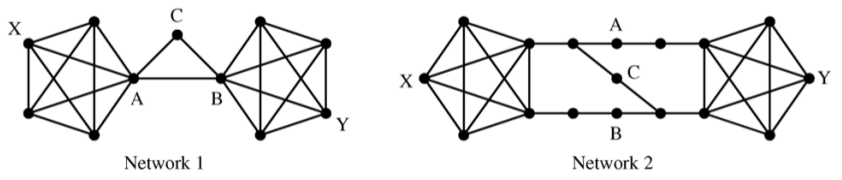
\includegraphics[width=0.7\linewidth]{./img/random_walk_betwenness_graph_newman.png}
				\caption{Utilité de la marche aléatoire pour le calcul de centralité intermédiaire selon Newman.}
				\label{fig:algo_brandes}
			\end{figure}
		    
		    \item<4-> Et bien d'autres...
		\end{itemize}
	\end{block}
\end{frame}

	\subsection{Méthodes d'approximation}

\begin{frame}
	\begin{block}{Quelques méthodes d'approximation}
		\begin{itemize}
		    \item Approximation grâce à un nombre restreint de n\oe uds sources (Brandes, 2007).
		    \item Approximation grâce à un nombre restreint de n\oe uds sources et l'utilisation de chemins de taille maximale (Alahakoon \textit{et al.}, 2011).
		\end{itemize}
	\end{block}
\end{frame}

\section{Les marches aléatoires}

	\subsection{Première hypothèse}
	
\begin{frame}
	\begin{figure}[htbp]
		\centering
		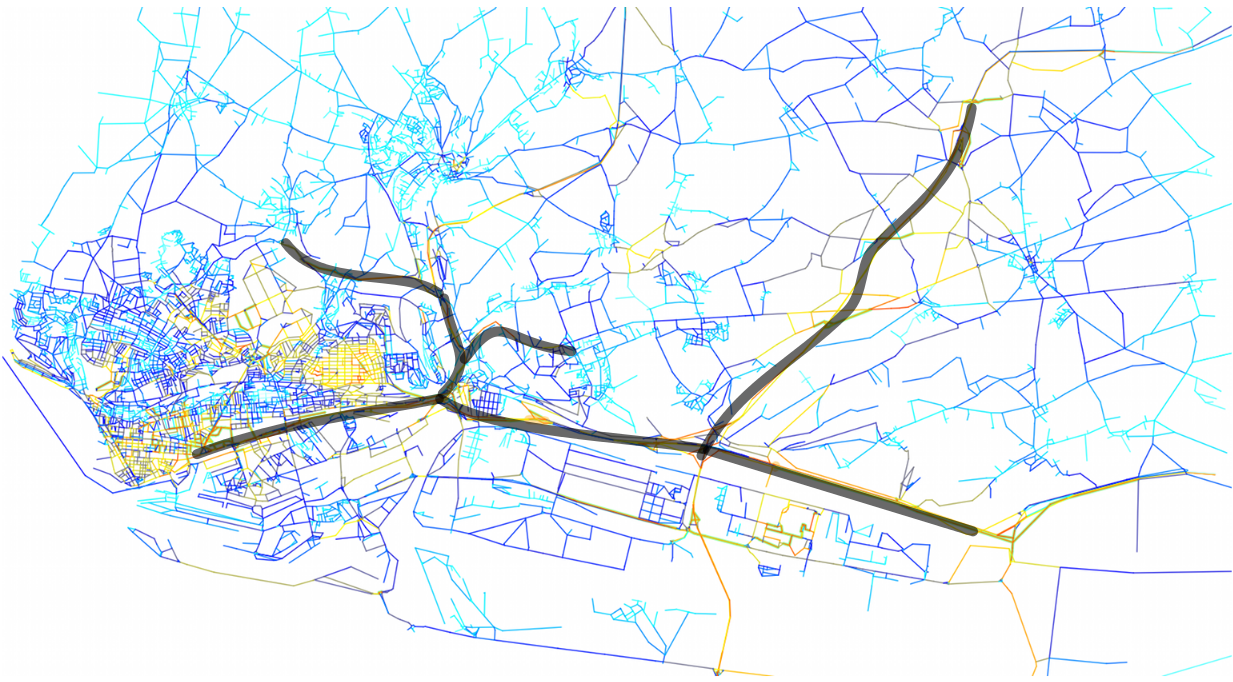
\includegraphics[width=1.\linewidth]{./img/marche_aleatoire_Nabaa_LeHavre.png}
		\caption{Résultat de la marche aléatoire sur le réseau viaire du Havre issu de la thèse de Michel Nabaa - du non emprunté en bleu clair au congestionné en rouge.}
		\label{fig:algo_brandes}
	\end{figure}
\end{frame}

\begin{frame}
	\begin{figure}[htbp]
		\centering
		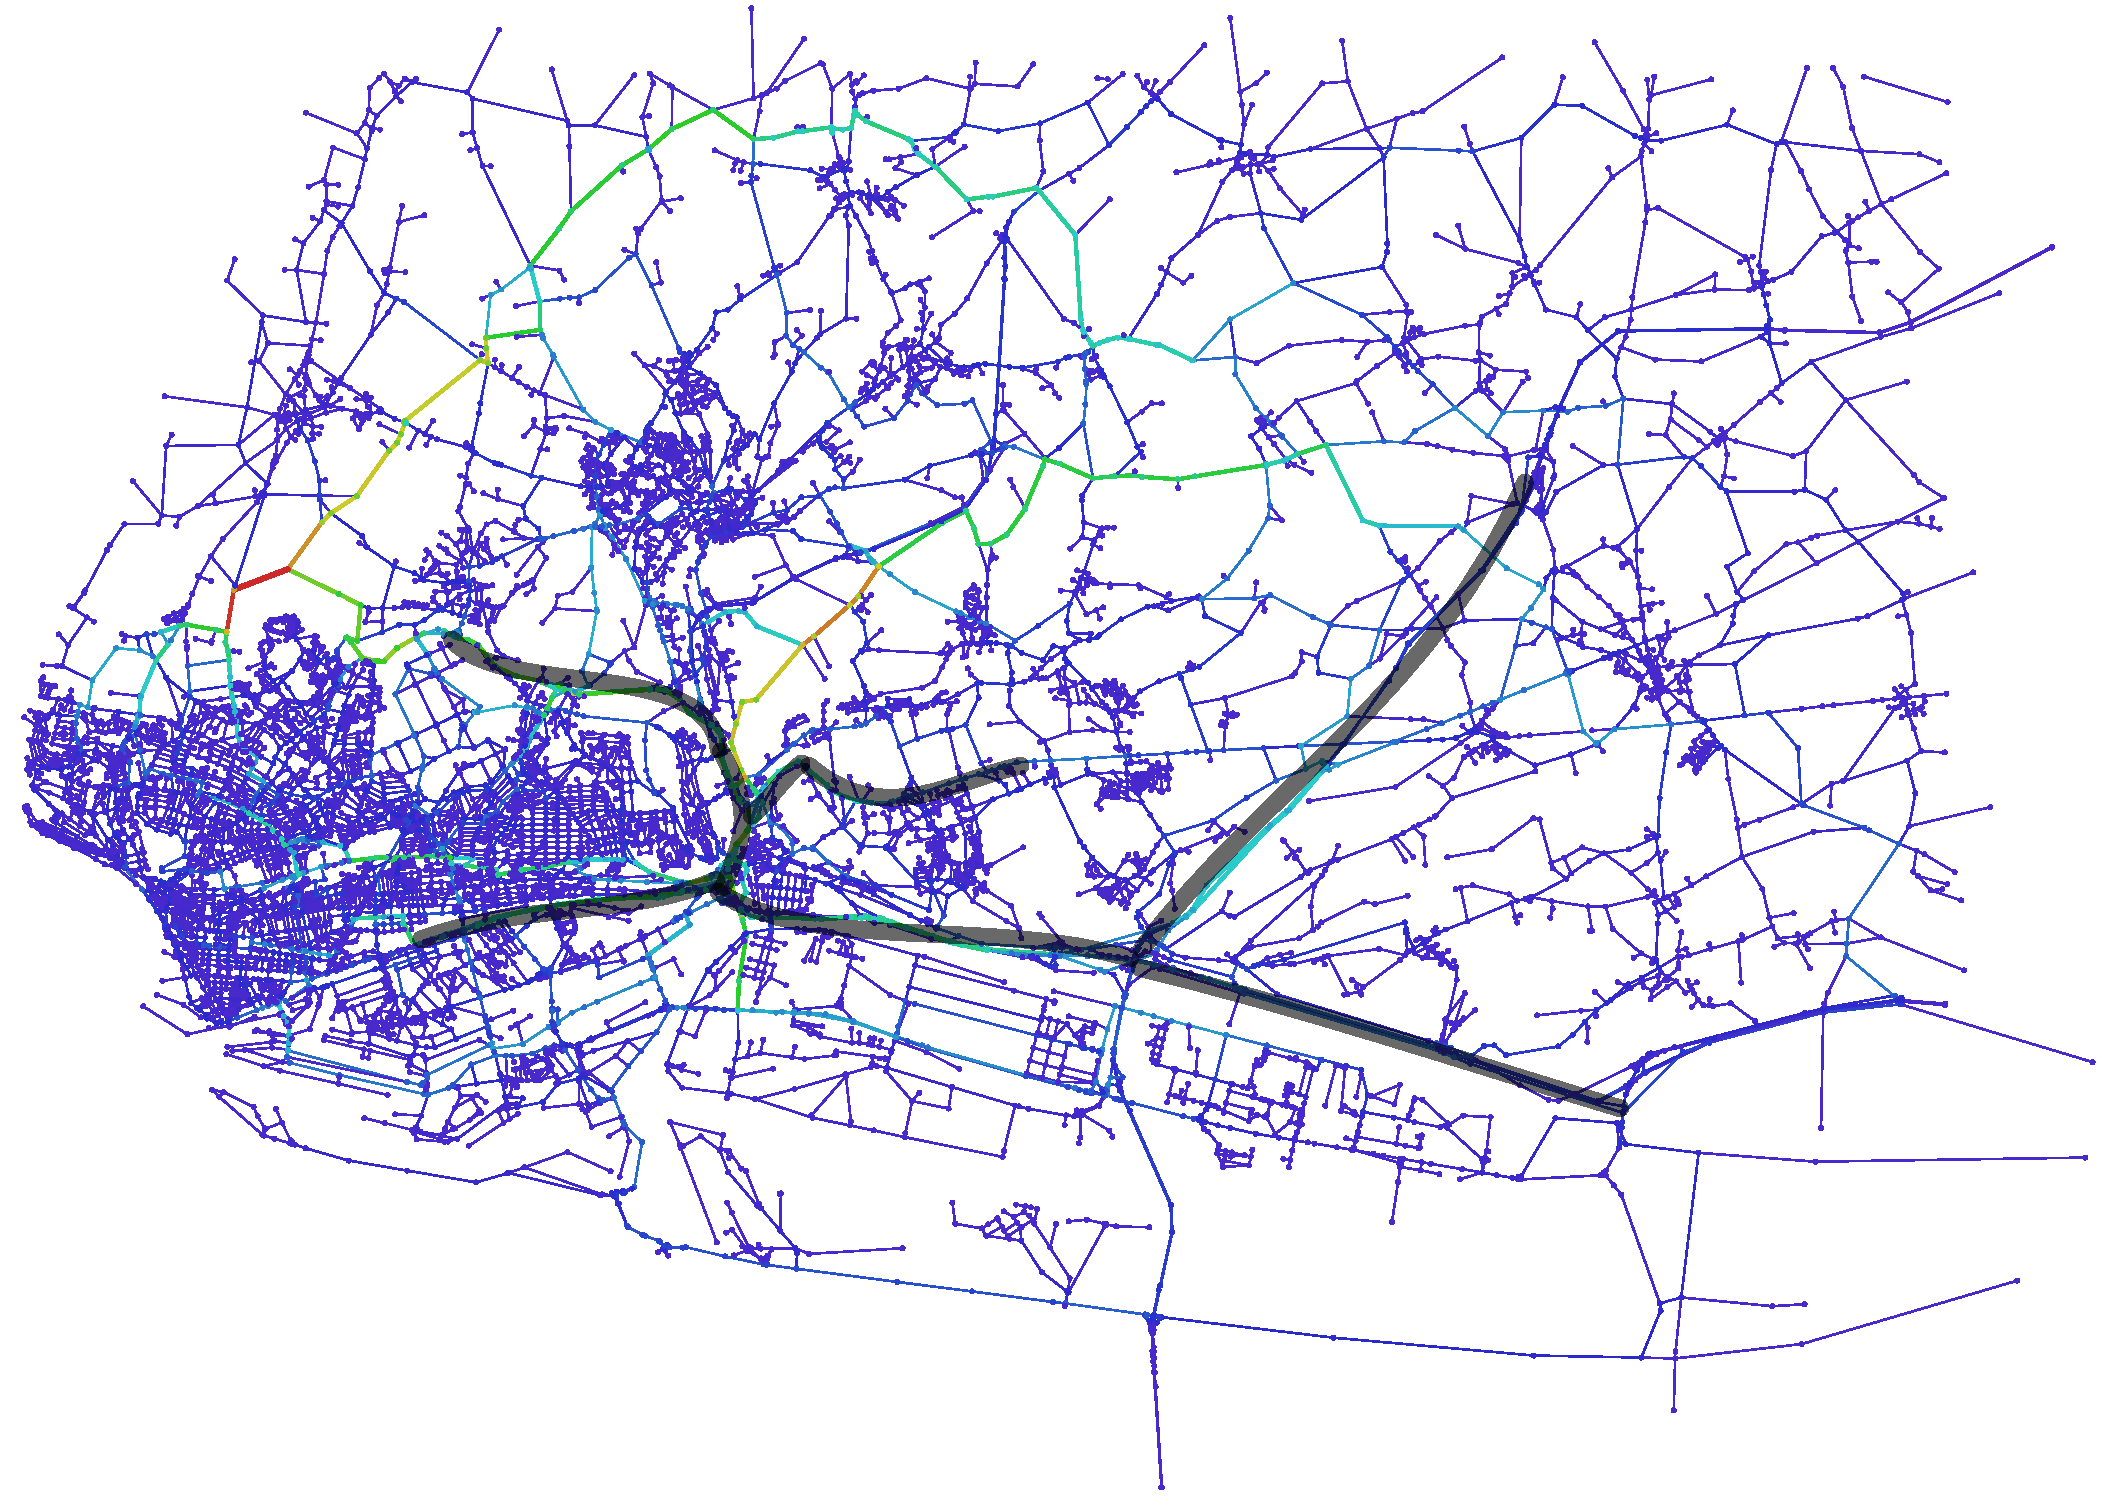
\includegraphics[width=0.8\linewidth]{./img/centralite_inter_noweight_Le_Havre.pdf}
		\caption{Résultat de la centralité intermédiaire sur le réseau viaire du Havre - de le centralité faible en bleu à la centralité forte en rouge.}
		\label{fig:algo_brandes}
	\end{figure}
\end{frame}
	
	\subsection{La marche aléatoire}
	
\begin{frame}{Le modèle}
	\begin{block}{Fonctionnement}
	    \begin{itemize}
	        \item Des entités effectuent une marche aléatoire, et utilisent un mécanisme tabou.
	        \item L'algorithme continue tant que la stabilité des valeurs n'est pas détectée.
	    \end{itemize}
	\end{block}
\end{frame}

	\subsection{Les résultats}
	
\begin{frame}
    \begin{figure}[htbp]
		\centering
		\subcaptionbox{Dorogovtsev et Mendes (1000 n\oe uds) - coefficient de corrélation de Pearson : 0.2405}[0.45\linewidth][c]{
			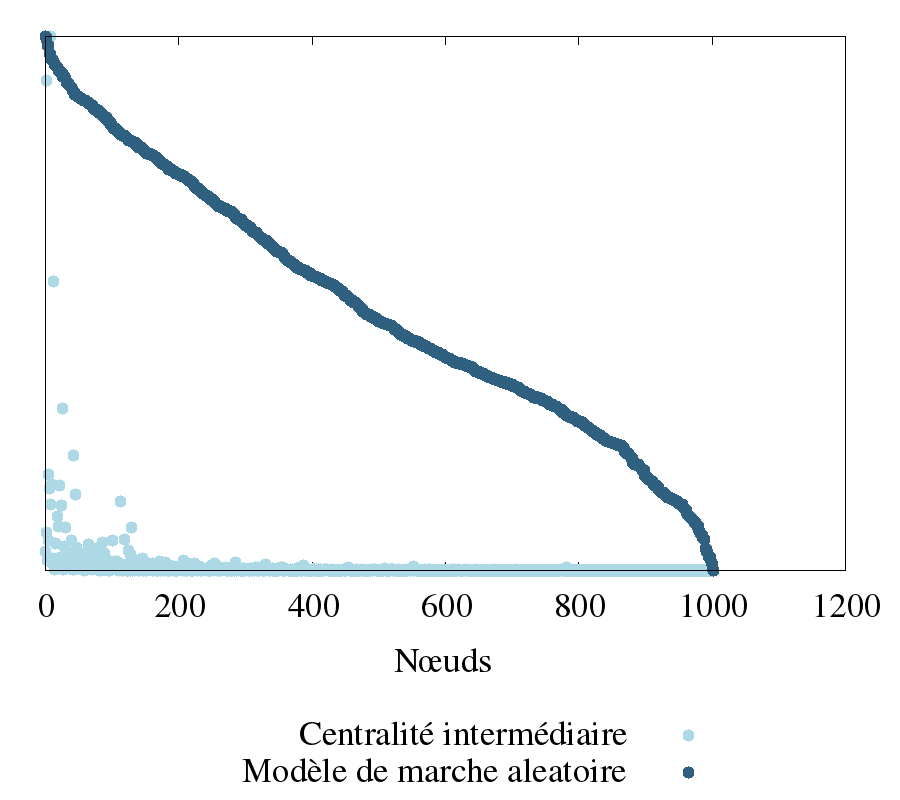
\includegraphics[width=0.45\linewidth]{./img/marche_aleatoire_dorogovstev_mendes.png}
		}
		\hfill
		\subcaptionbox{Small-world (1000 n\oe uds, $k=2$ et $\beta=0.5$) - coefficient de corrélation de Pearson : 0.2783}[0.45\linewidth][c]{
			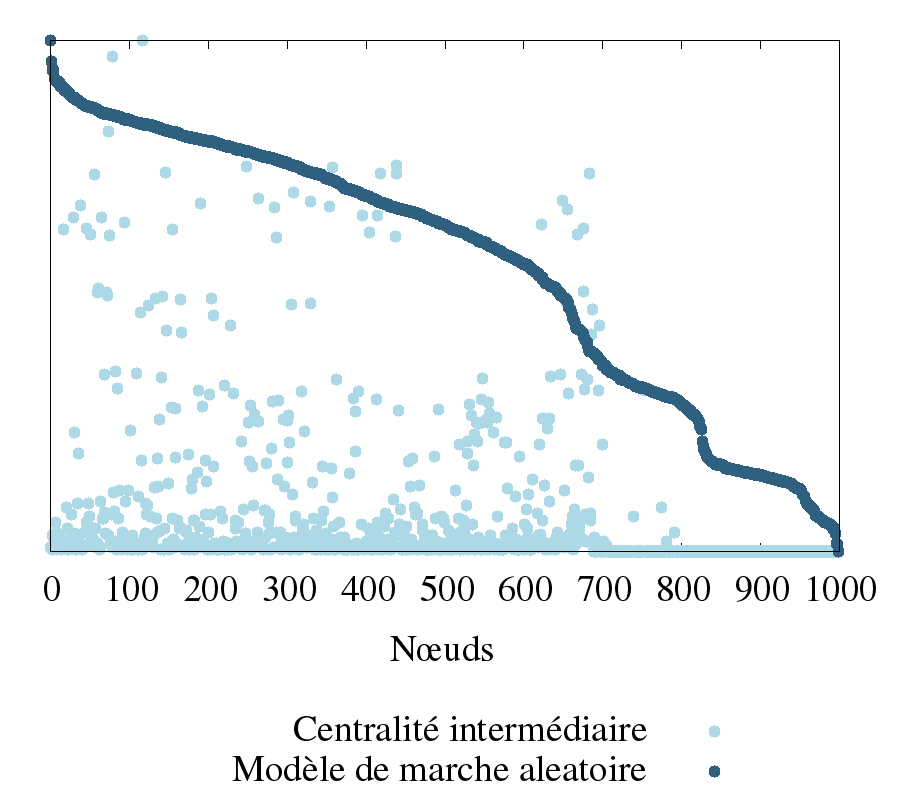
\includegraphics[width=0.45\linewidth]{./img/marche_aleatoire_small_world_1000_2_0_5.png}
		}
		\caption{En abscisses, il s'agit de la liste ordonnée des n\oe uds selon la mesure de notre modèle; en ordonnées, les points sont situés en fonction du score obtenu par l'une ou l'autre des mesures.}
		\label{fig:graphiques_random_walk_1}
	\end{figure}
\end{frame}

\begin{frame}
    \begin{figure}[htbp]
		\centering
		\subcaptionbox{Le Havre (11736  n\oe uds) - coefficient de corrélation de Pearson : 0.3043}[0.45\linewidth][c]{
			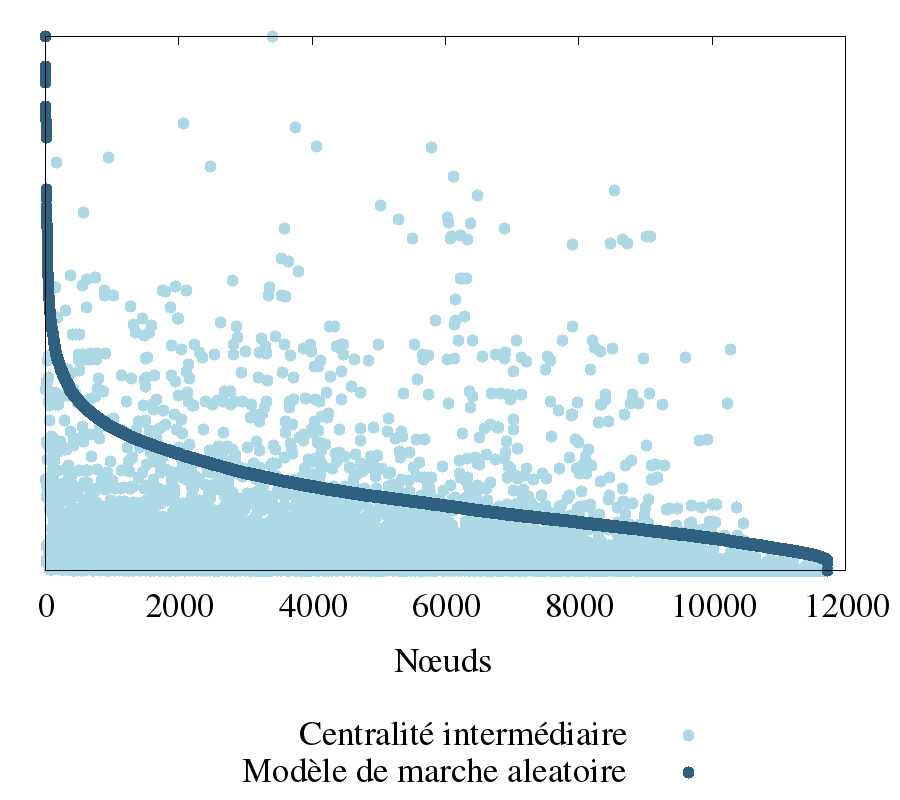
\includegraphics[width=0.45\linewidth]{./img/marche_aleatoire_le_havre.png}
		}
		\caption{En abscisses, il s'agit de la liste ordonnée des n\oe uds selon la mesure de notre modèle; en ordonnées, les points sont situés en fonction du score obtenu par l'une ou l'autre des mesures.}
		\label{fig:graphiques_random_walk_2}
	\end{figure}
\end{frame}

\section{La centralité intermédiaire avec pivots}

	\subsection{Le modèle}

\begin{frame}
	\begin{block}{Intuition inspirée du modèle de Brandes (2007)}
		Le modèle de Brandes montre que :
		\begin{itemize}
			\item Un ensemble de n\oe uds pivots suffisamment grand permet une corrélation acceptable.
			\pause \item Certaines paires seraient plus pertinentes que d'autres.
		\end{itemize}
		\pause Ainsi, pourquoi ne pas sélectionner aléatoirement les n\oe uds composants des paires?
	\end{block}
\end{frame}

\begin{frame}
	\begin{block}{Le modèle des pivots}
		\begin{itemize}
		    \item Un processus maître sélectionne aléatoirement les n\oe uds des paires.
		    \pause \item Des entités doivent résoudre des plus courts chemins entre les n\oe uds de ces paires.
		\end{itemize}
		\pause Mais quel comportement au sein de l'entité?
	\end{block}
\end{frame}

	\subsection{Les entités effectuant des marches aléatoires}

\begin{frame}
	\begin{block}{Fonctionnement}
		\begin{itemize}
		    \item L'entité commence sur le n\oe ud source d'une paire.
		    \item Elle doit ensuite se déplacer de n\oe ud en n\oe ud par sélection aléatoire.
		    \item Elle s'arrête lorsqu'elle atteint le n\oe ud cible.
		\end{itemize}
	\end{block}
\end{frame}

\begin{frame}
    \begin{figure}[htbp]
		\centering
		\subcaptionbox{Dorogovtsev et Mendes (1000 n\oe uds) - coefficient de corrélation de Pearson : 0.9668}[0.3\linewidth][c]{
			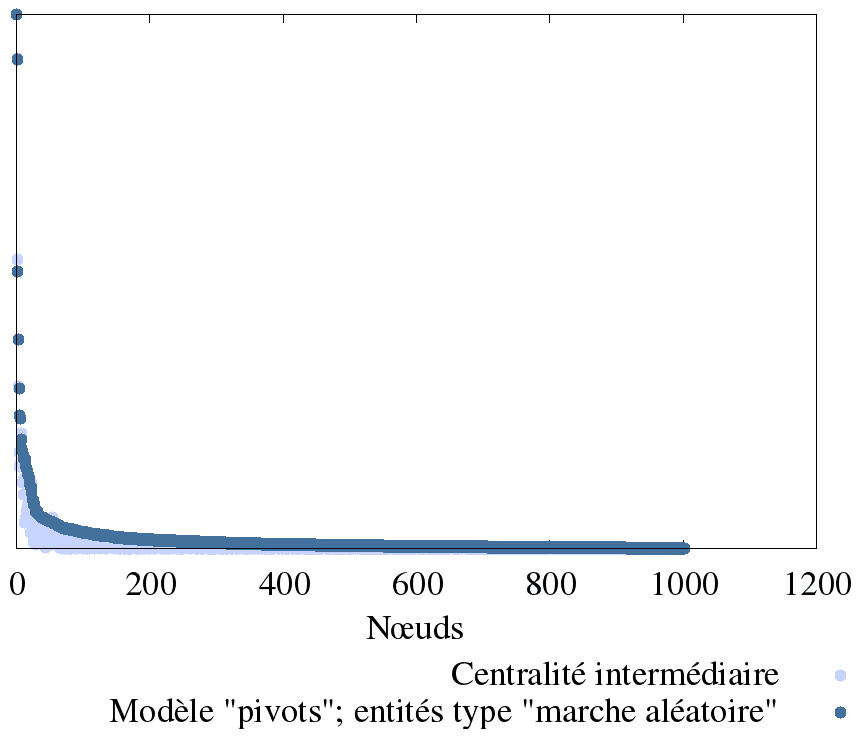
\includegraphics[width=0.3\linewidth]{./img/pivots_marche_aleatoire_dorogovstev_mendes.png}
		}
		\hfill
		\subcaptionbox{Grille (10000 n\oe uds) - coefficient de corrélation de Pearson : 0.9368}[0.3\linewidth][c]{
			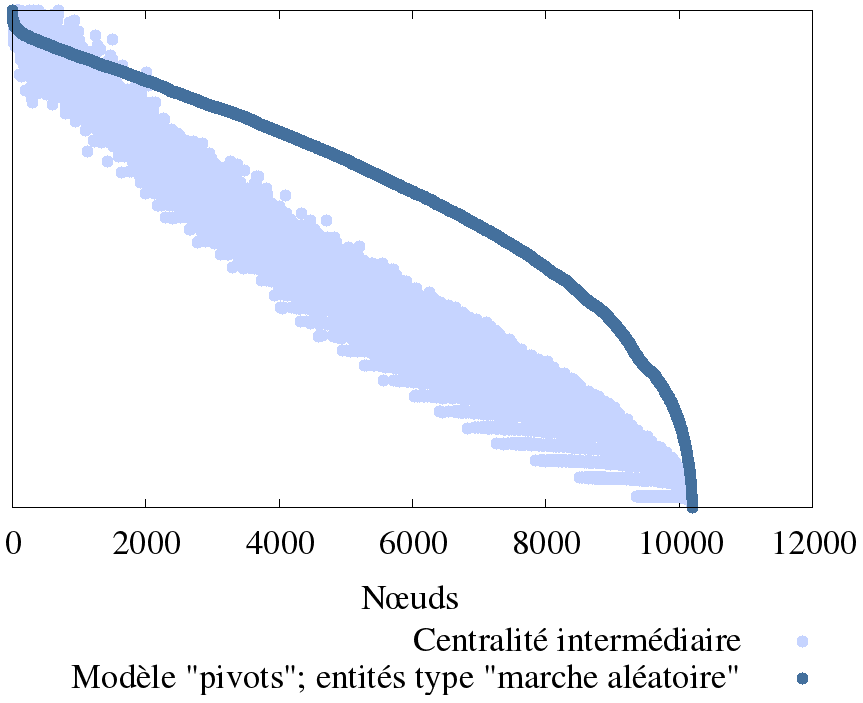
\includegraphics[width=0.3\linewidth]{./img/pivots_marche_aleatoire_grille_10000.png}
		}
		\hfill
		\subcaptionbox{Small-world (1000 n\oe uds, $k=2$ et $\beta=0.5$) - coefficient de corrélation de Pearson : 0.9737}[0.3\linewidth][c]{
			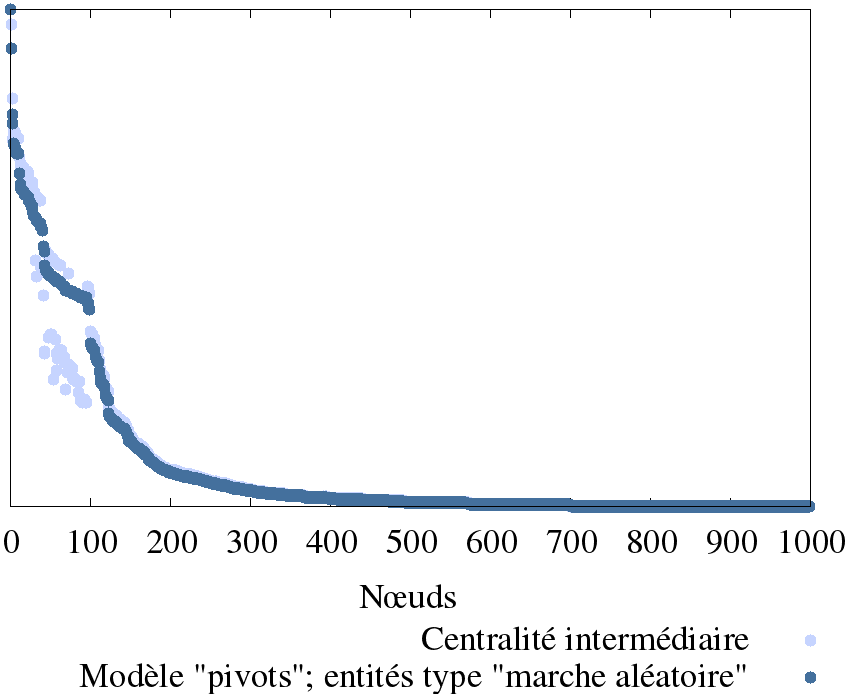
\includegraphics[width=0.3\linewidth]{./img/pivots_marche_aleatoire_small_world_1000_2_0_5.png}
		}
		\caption{En abscisses, il s'agit de la liste ordonnée des n\oe uds selon la mesure de notre modèle; en ordonnées, les points sont situés en fonction du score obtenu par l'une ou l'autre des mesures.}
		\label{fig:graphiques_pivots_random_walk_1}
	\end{figure}
\end{frame}

\begin{frame}
    \begin{figure}[htbp]
		\centering
		\subcaptionbox{Small-world (1000 n\oe uds, $k=4$ et $\beta=0.01$) - coefficient de corrélation de Pearson : 0.7964}[0.49\linewidth][c]{
			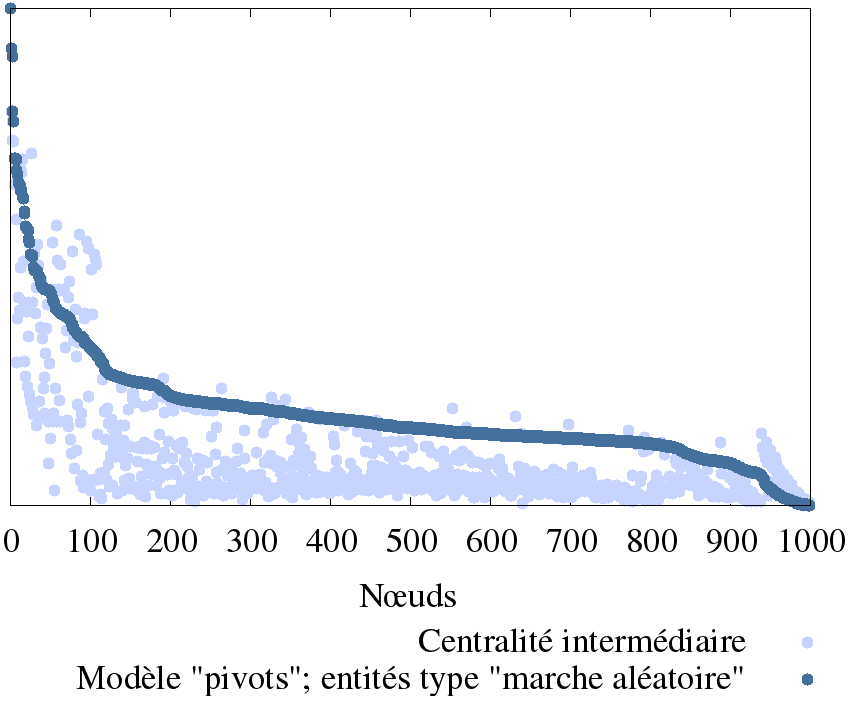
\includegraphics[width=0.49\linewidth]{./img/pivots_marche_aleatoire_small_world_1000_4_0_01.png}
		}
		\caption{En abscisses, il s'agit de la liste ordonnée des n\oe uds selon la mesure de notre modèle; en ordonnées, les points sont situés en fonction du score obtenu par l'une ou l'autre des mesures.}
		\label{fig:graphiques_pivots_random_walk_2}
	\end{figure}
\end{frame}


\begin{frame}
    \begin{figure}[htbp]
		\centering
		\subcaptionbox{Le Havre (11736  n\oe uds) - coefficient de corrélation de Pearson : 0.6481}[0.49\linewidth][c]{
			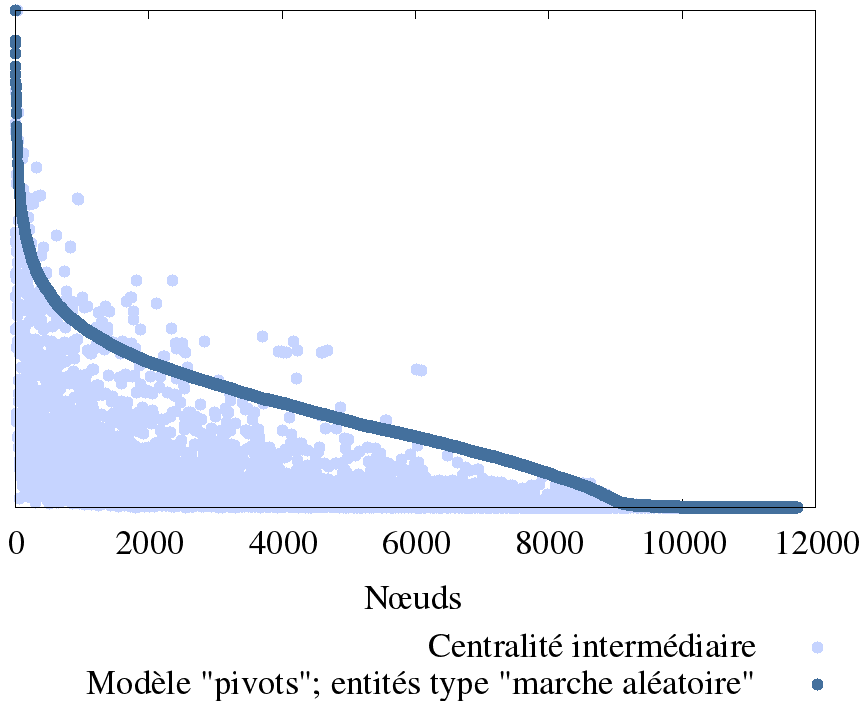
\includegraphics[width=0.49\linewidth]{./img/pivots_marche_aleatoire_le_havre.png}
		}
		\hfill
		\subcaptionbox{Rouen (17442  n\oe uds) - coefficient de corrélation de Pearson : 0.5805}[0.49\linewidth][c]{
			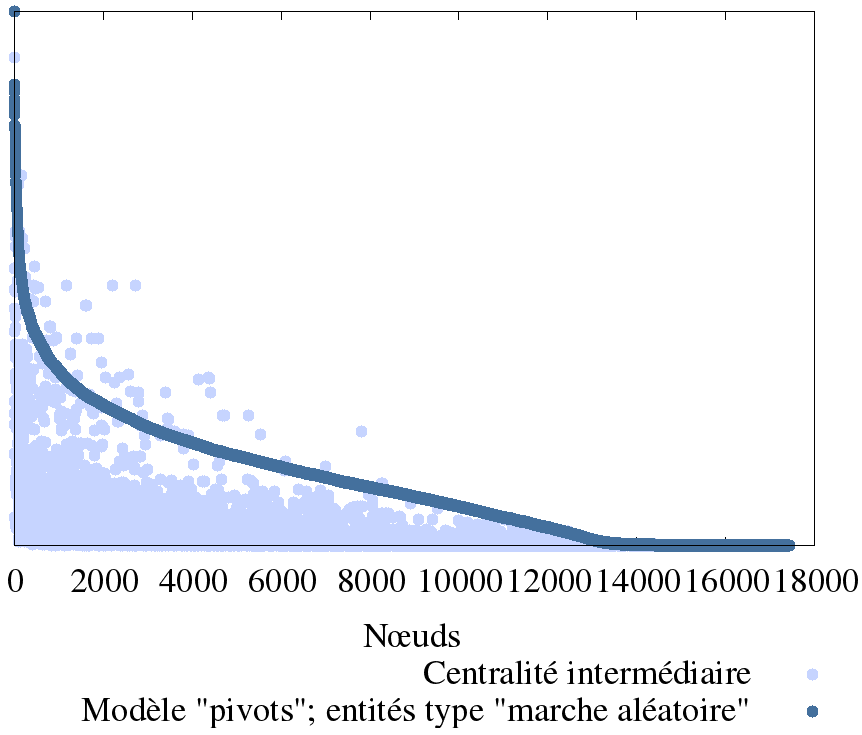
\includegraphics[width=0.49\linewidth]{./img/pivots_marche_aleatoire_rouen.png}
		}
		\caption{En abscisses, il s'agit de la liste ordonnée des n\oe uds selon la mesure de notre modèle; en ordonnées, les points sont situés en fonction du score obtenu par l'une ou l'autre des mesures.}
		\label{fig:graphiques_pivots_random_walk_2}
	\end{figure}
\end{frame}

	\subsection{Les entités utilisant A$^*$}

\begin{frame}
	\begin{block}{Fonctionnement}
		\begin{itemize}
		    \item Volonté de se rapprocher des plus courts chemins.
		    \item Le chemin définit par l'entité est la solution d'une exécution de A$^*$.
		\end{itemize}
	\end{block}
\end{frame}

\begin{frame}
	\begin{block}{Fonctionnement}
		\begin{itemize}
		    \item Nécessite une heuristique monotone et admissible pour calculer un plus court chemin.
		    \item Résultats uniquement sur Le Havre et Rouen.
		    \item Utilisation de la distance euclidienne comme heuristique.
		\end{itemize}
	\end{block}
\end{frame}

\begin{frame}
	\begin{figure}[htbp]
		\centering
		\subcaptionbox{Le Havre (11736  n\oe uds) - coefficient de corrélation de Pearson : 0.9817}[0.47\linewidth][c]{
			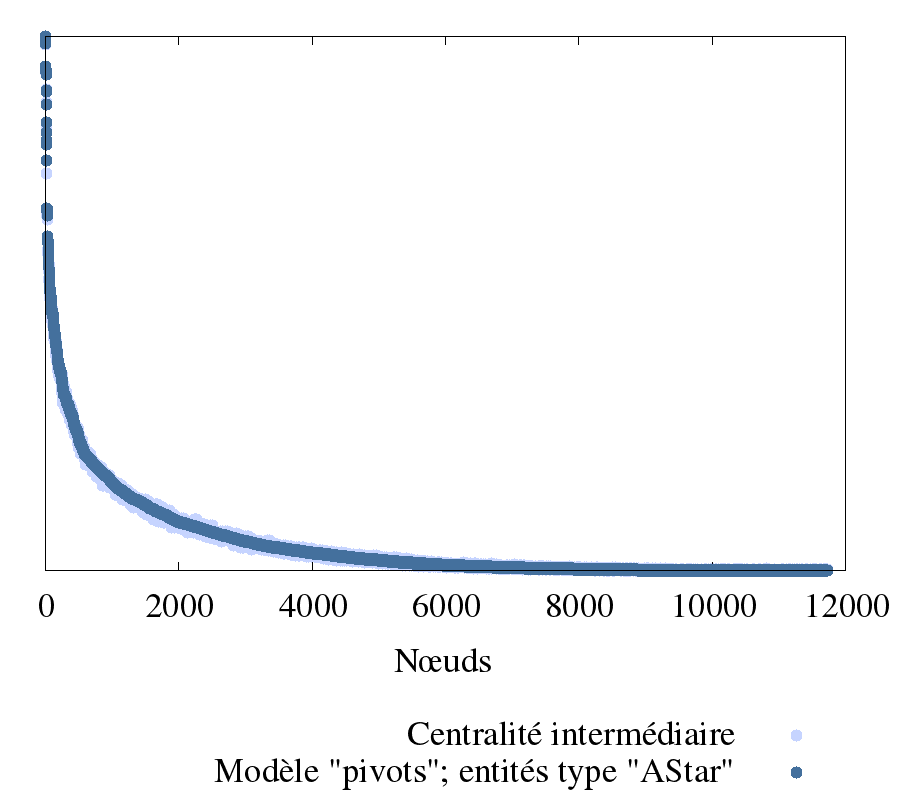
\includegraphics[width=0.47\linewidth]{./img/pivots_astar_le_havre.png}
		}
		\hfill
		\subcaptionbox{Rouen (17442 n\oe uds) - coefficient de corrélation de Pearson : 0.9834}[0.47\linewidth][c]{
			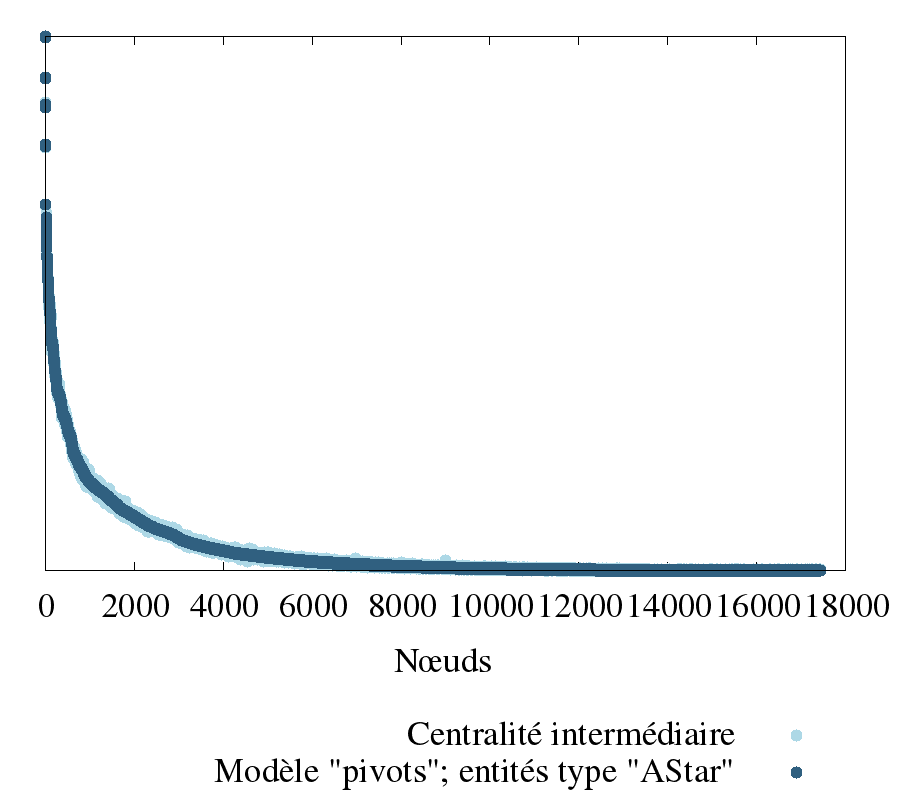
\includegraphics[width=0.47\linewidth]{./img/pivots_astar_rouen.png}
		}
		\caption{En abscisses, il s'agit de la liste ordonnée des n\oe uds selon la mesure de notre modèle; en ordonnées, les points sont situés en fonction du score obtenu par l'une ou l'autre des mesures.}
		\label{fig:graphiques_pivots_astar}
	\end{figure}
\end{frame}

	\subsection{Les entités fourmis}

\begin{frame}
	\begin{block}{Fonctionnement}
		\begin{itemize}
		    \item Inspiré du modèle de Dorigo \textit{et al.}, 1992. 
		    \item Modèle d'optimisation à l'aide d'un mécanisme de stigmergie.
		    \item Robuste à la dynamique d'un graphe.
		\end{itemize}
	\end{block}
\end{frame}

\begin{frame}
	\begin{block}{Fonctionnement}
		\begin{itemize}
		    \item L'entité se déplace selon une marche aléatoire biaisée par des phéromones selon :
$$
	p_i = \frac{\tau_{i}^{\alpha}\cdot \eta_{i}^{\beta}}{ \sum\limits_{j=1}^{k}\tau_{j}^{\alpha}\cdot \eta_{j}^{\beta}}
$$

		    \pause \item Elle pose des phéromones sur son chemin, en fonction de la distance parcourue selon :
$$
	\tau_s = \tau_s + \frac{Q}{\text{l(C)}}
$$
		\end{itemize}
	\end{block}
\end{frame}

\begin{frame}
	\begin{block}{Fonctionnement}
		\begin{itemize}
		    \item Le processus maître gère un mécanisme d'évaporation de la phéromone.
		    \item Il gère également l'ensemble de la colonie et les paires de n\oe uds.
		\end{itemize}
	\end{block}
\end{frame}

\begin{frame}
	\begin{figure}[htbp]
		\centering
		\subcaptionbox{Grille (100 n\oe uds)}[0.47\linewidth][c]{
			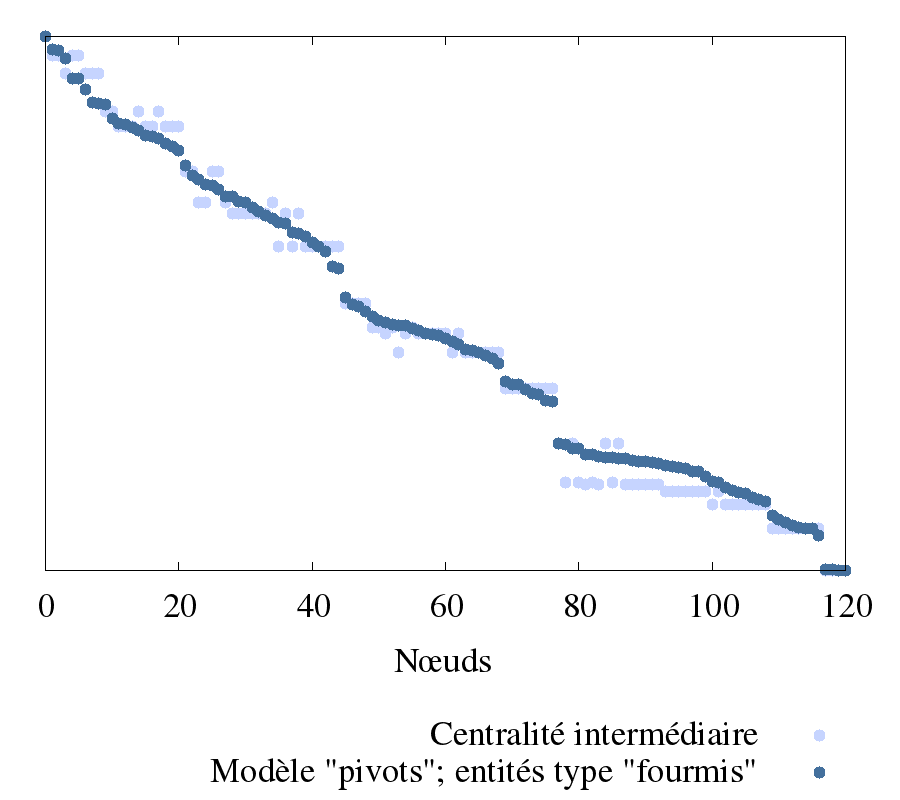
\includegraphics[width=0.47\linewidth]{./img/pivots_fourmis_grille_10.png}
		}
		\caption{En abscisses, il s'agit de la liste ordonnée des n\oe uds selon la mesure de notre modèle; en ordonnées, les points sont situés en fonction du score obtenu par l'une ou l'autre des mesures.}
		\label{fig:graphiques_pivots_astar}
	\end{figure}
\end{frame}

\section{Conclusion et perspectives}

\begin{frame}
	\begin{block}{Conclusion}
		\begin{itemize}
		    \item L'essai manqué de la marche aléatoire classique.
		    \item L'approche de la centralité intermédiaire avec pivots.
		    \item Un résultat prometteur pour l'entité fourmi.
		\end{itemize}
	\end{block}
\end{frame}

\begin{frame}
	\begin{block}{Perspectives}
		\begin{itemize}
		    \item Continuer l'implémentation de l'entité fourmi.
		    \item Rechercher une méthode plus élaborées de sélection des paires.
		    \item Définir le nombre de paires nécessaires pour obtenir une corrélation "correcte".
		    \item Distribuer l'algorithme.
		\end{itemize}
	\end{block}
\end{frame}

\begin{frame}
     \begin{center}
         Merci de votre attention.
         
         Souhaitez-vous poser des questions?
     \end{center}
\end{frame}

\end{document}